% Options for packages loaded elsewhere
% Options for packages loaded elsewhere
\PassOptionsToPackage{unicode}{hyperref}
\PassOptionsToPackage{hyphens}{url}
\PassOptionsToPackage{dvipsnames,svgnames,x11names}{xcolor}
%
\documentclass[
  letterpaper,
  DIV=11,
  numbers=noendperiod]{scrartcl}
\usepackage{xcolor}
\usepackage[margin=1in]{geometry}
\usepackage{amsmath,amssymb}
\setcounter{secnumdepth}{5}
\usepackage{iftex}
\ifPDFTeX
  \usepackage[T1]{fontenc}
  \usepackage[utf8]{inputenc}
  \usepackage{textcomp} % provide euro and other symbols
\else % if luatex or xetex
  \usepackage{unicode-math} % this also loads fontspec
  \defaultfontfeatures{Scale=MatchLowercase}
  \defaultfontfeatures[\rmfamily]{Ligatures=TeX,Scale=1}
\fi
\usepackage{lmodern}
\ifPDFTeX\else
  % xetex/luatex font selection
\fi
% Use upquote if available, for straight quotes in verbatim environments
\IfFileExists{upquote.sty}{\usepackage{upquote}}{}
\IfFileExists{microtype.sty}{% use microtype if available
  \usepackage[]{microtype}
  \UseMicrotypeSet[protrusion]{basicmath} % disable protrusion for tt fonts
}{}
\makeatletter
\@ifundefined{KOMAClassName}{% if non-KOMA class
  \IfFileExists{parskip.sty}{%
    \usepackage{parskip}
  }{% else
    \setlength{\parindent}{0pt}
    \setlength{\parskip}{6pt plus 2pt minus 1pt}}
}{% if KOMA class
  \KOMAoptions{parskip=half}}
\makeatother
% Make \paragraph and \subparagraph free-standing
\makeatletter
\ifx\paragraph\undefined\else
  \let\oldparagraph\paragraph
  \renewcommand{\paragraph}{
    \@ifstar
      \xxxParagraphStar
      \xxxParagraphNoStar
  }
  \newcommand{\xxxParagraphStar}[1]{\oldparagraph*{#1}\mbox{}}
  \newcommand{\xxxParagraphNoStar}[1]{\oldparagraph{#1}\mbox{}}
\fi
\ifx\subparagraph\undefined\else
  \let\oldsubparagraph\subparagraph
  \renewcommand{\subparagraph}{
    \@ifstar
      \xxxSubParagraphStar
      \xxxSubParagraphNoStar
  }
  \newcommand{\xxxSubParagraphStar}[1]{\oldsubparagraph*{#1}\mbox{}}
  \newcommand{\xxxSubParagraphNoStar}[1]{\oldsubparagraph{#1}\mbox{}}
\fi
\makeatother

\usepackage{color}
\usepackage{fancyvrb}
\newcommand{\VerbBar}{|}
\newcommand{\VERB}{\Verb[commandchars=\\\{\}]}
\DefineVerbatimEnvironment{Highlighting}{Verbatim}{commandchars=\\\{\}}
% Add ',fontsize=\small' for more characters per line
\usepackage{framed}
\definecolor{shadecolor}{RGB}{241,243,245}
\newenvironment{Shaded}{\begin{snugshade}}{\end{snugshade}}
\newcommand{\AlertTok}[1]{\textcolor[rgb]{0.68,0.00,0.00}{#1}}
\newcommand{\AnnotationTok}[1]{\textcolor[rgb]{0.37,0.37,0.37}{#1}}
\newcommand{\AttributeTok}[1]{\textcolor[rgb]{0.40,0.45,0.13}{#1}}
\newcommand{\BaseNTok}[1]{\textcolor[rgb]{0.68,0.00,0.00}{#1}}
\newcommand{\BuiltInTok}[1]{\textcolor[rgb]{0.00,0.23,0.31}{#1}}
\newcommand{\CharTok}[1]{\textcolor[rgb]{0.13,0.47,0.30}{#1}}
\newcommand{\CommentTok}[1]{\textcolor[rgb]{0.37,0.37,0.37}{#1}}
\newcommand{\CommentVarTok}[1]{\textcolor[rgb]{0.37,0.37,0.37}{\textit{#1}}}
\newcommand{\ConstantTok}[1]{\textcolor[rgb]{0.56,0.35,0.01}{#1}}
\newcommand{\ControlFlowTok}[1]{\textcolor[rgb]{0.00,0.23,0.31}{\textbf{#1}}}
\newcommand{\DataTypeTok}[1]{\textcolor[rgb]{0.68,0.00,0.00}{#1}}
\newcommand{\DecValTok}[1]{\textcolor[rgb]{0.68,0.00,0.00}{#1}}
\newcommand{\DocumentationTok}[1]{\textcolor[rgb]{0.37,0.37,0.37}{\textit{#1}}}
\newcommand{\ErrorTok}[1]{\textcolor[rgb]{0.68,0.00,0.00}{#1}}
\newcommand{\ExtensionTok}[1]{\textcolor[rgb]{0.00,0.23,0.31}{#1}}
\newcommand{\FloatTok}[1]{\textcolor[rgb]{0.68,0.00,0.00}{#1}}
\newcommand{\FunctionTok}[1]{\textcolor[rgb]{0.28,0.35,0.67}{#1}}
\newcommand{\ImportTok}[1]{\textcolor[rgb]{0.00,0.46,0.62}{#1}}
\newcommand{\InformationTok}[1]{\textcolor[rgb]{0.37,0.37,0.37}{#1}}
\newcommand{\KeywordTok}[1]{\textcolor[rgb]{0.00,0.23,0.31}{\textbf{#1}}}
\newcommand{\NormalTok}[1]{\textcolor[rgb]{0.00,0.23,0.31}{#1}}
\newcommand{\OperatorTok}[1]{\textcolor[rgb]{0.37,0.37,0.37}{#1}}
\newcommand{\OtherTok}[1]{\textcolor[rgb]{0.00,0.23,0.31}{#1}}
\newcommand{\PreprocessorTok}[1]{\textcolor[rgb]{0.68,0.00,0.00}{#1}}
\newcommand{\RegionMarkerTok}[1]{\textcolor[rgb]{0.00,0.23,0.31}{#1}}
\newcommand{\SpecialCharTok}[1]{\textcolor[rgb]{0.37,0.37,0.37}{#1}}
\newcommand{\SpecialStringTok}[1]{\textcolor[rgb]{0.13,0.47,0.30}{#1}}
\newcommand{\StringTok}[1]{\textcolor[rgb]{0.13,0.47,0.30}{#1}}
\newcommand{\VariableTok}[1]{\textcolor[rgb]{0.07,0.07,0.07}{#1}}
\newcommand{\VerbatimStringTok}[1]{\textcolor[rgb]{0.13,0.47,0.30}{#1}}
\newcommand{\WarningTok}[1]{\textcolor[rgb]{0.37,0.37,0.37}{\textit{#1}}}

\usepackage{longtable,booktabs,array}
\newcounter{none} % for unnumbered tables
\usepackage{calc} % for calculating minipage widths
% Correct order of tables after \paragraph or \subparagraph
\usepackage{etoolbox}
\makeatletter
\patchcmd\longtable{\par}{\if@noskipsec\mbox{}\fi\par}{}{}
\makeatother
% Allow footnotes in longtable head/foot
\IfFileExists{footnotehyper.sty}{\usepackage{footnotehyper}}{\usepackage{footnote}}
\makesavenoteenv{longtable}
\usepackage{graphicx}
\makeatletter
\newsavebox\pandoc@box
\newcommand*\pandocbounded[1]{% scales image to fit in text height/width
  \sbox\pandoc@box{#1}%
  \Gscale@div\@tempa{\textheight}{\dimexpr\ht\pandoc@box+\dp\pandoc@box\relax}%
  \Gscale@div\@tempb{\linewidth}{\wd\pandoc@box}%
  \ifdim\@tempb\p@<\@tempa\p@\let\@tempa\@tempb\fi% select the smaller of both
  \ifdim\@tempa\p@<\p@\scalebox{\@tempa}{\usebox\pandoc@box}%
  \else\usebox{\pandoc@box}%
  \fi%
}
% Set default figure placement to htbp
\def\fps@figure{htbp}
\makeatother





\setlength{\emergencystretch}{3em} % prevent overfull lines

\providecommand{\tightlist}{%
  \setlength{\itemsep}{0pt}\setlength{\parskip}{0pt}}



 


\KOMAoption{captions}{tableheading}
\makeatletter
\@ifpackageloaded{caption}{}{\usepackage{caption}}
\AtBeginDocument{%
\ifdefined\contentsname
  \renewcommand*\contentsname{Table of contents}
\else
  \newcommand\contentsname{Table of contents}
\fi
\ifdefined\listfigurename
  \renewcommand*\listfigurename{List of Figures}
\else
  \newcommand\listfigurename{List of Figures}
\fi
\ifdefined\listtablename
  \renewcommand*\listtablename{List of Tables}
\else
  \newcommand\listtablename{List of Tables}
\fi
\ifdefined\figurename
  \renewcommand*\figurename{Figure}
\else
  \newcommand\figurename{Figure}
\fi
\ifdefined\tablename
  \renewcommand*\tablename{Table}
\else
  \newcommand\tablename{Table}
\fi
}
\@ifpackageloaded{float}{}{\usepackage{float}}
\floatstyle{ruled}
\@ifundefined{c@chapter}{\newfloat{codelisting}{h}{lop}}{\newfloat{codelisting}{h}{lop}[chapter]}
\floatname{codelisting}{Listing}
\newcommand*\listoflistings{\listof{codelisting}{List of Listings}}
\makeatother
\makeatletter
\makeatother
\makeatletter
\@ifpackageloaded{caption}{}{\usepackage{caption}}
\@ifpackageloaded{subcaption}{}{\usepackage{subcaption}}
\makeatother
\usepackage{bookmark}
\IfFileExists{xurl.sty}{\usepackage{xurl}}{} % add URL line breaks if available
\urlstyle{same}
\hypersetup{
  pdftitle={Skintone Beauty Recommender},
  pdfauthor={Sheriann McLarty},
  colorlinks=true,
  linkcolor={blue},
  filecolor={Maroon},
  citecolor={Blue},
  urlcolor={Blue},
  pdfcreator={LaTeX via pandoc}}


\title{Skintone Beauty Recommender}
\usepackage{etoolbox}
\makeatletter
\providecommand{\subtitle}[1]{% add subtitle to \maketitle
  \apptocmd{\@title}{\par {\large #1 \par}}{}{}
}
\makeatother
\subtitle{A Hybrid Clean Beauty Recommender for Ingredient Safety, Skin
Type, and Skin Tone Compatibility}
\author{Sheriann McLarty}
\date{2026-05-01}
\begin{document}
\maketitle

\renewcommand*\contentsname{Table of contents}
{
\setcounter{tocdepth}{3}
\tableofcontents
}

\section{Abstract}\label{abstract}

This capstone presents Skintone, a safety-constrained hybrid clean
beauty recommender system designed to support ingredient safety, skin
tone compatibility, and personalized product ranking for melanin-rich
users. Traditional beauty recommender systems prioritize ratings,
engagement, and popularity, but these signals alone do not adequately
address whether a product is safe for a user's ingredient concerns or
whether it performs well across different skin tones. This gap
disproportionately affects melanin-rich consumers, who may experience
product mismatch, irritation, oxidation, flashback, or limited
representation in review data.

Skintone builds on a bias-adjusted collaborative filtering model and
extends it with a filter-first ingredient safety layer using the
European Commission's CosIng regulatory database, nut allergen
detection, sensitive skin and eczema screening based on review language,
skin type preference ranking, and review-based skin tone compatibility
signals. The system is implemented as a Streamlit web application using
Sephora review and product metadata. Results demonstrate that safety
constraints can be enforced prior to personalization while still
producing useful recommendations, and that review-based skin tone
signals provide meaningful evidence of product compatibility for
melanin-rich users.

\begin{center}\rule{0.5\linewidth}{0.5pt}\end{center}

\section{1. Introduction}\label{introduction}

Beauty recommendation systems are often presented as neutral ranking
tools that surface top products based on ratings or similar-user
behavior. However, beauty products interact directly with the skin and
can carry ingredient risks, sensitivity concerns, and tone-specific
performance issues that average ratings do not capture. A high average
rating does not guarantee that a product is safe, suitable, or
compatible for every consumer.

For melanin-rich users in particular, many products perform differently
due to undertone mismatch, oxidation, flashback, white cast, or lack of
shade inclusivity. These performance issues are rarely reflected in
existing recommendation systems, which tend to optimize for engagement
and popularity without considering ingredient safety or skin tone
compatibility.

At the same time, regulatory protection for cosmetic ingredient safety
is significantly weaker in the United States than in the European Union.
While the EU's CosIng database identifies over 2,100 prohibited or
restricted substances, the United States has banned or restricted fewer
than 30 cosmetic ingredients under the Modernization of Cosmetics
Regulation Act (MoCRA). This regulatory gap places a greater burden on
consumers to evaluate product safety independently --- a burden that
falls disproportionately on melanin-rich consumers who are more likely
to be targeted with products containing potentially harmful ingredients.

Skintone addresses this gap by introducing a safety-constrained, hybrid
recommender architecture that prioritizes ingredient and allergen
filtering before personalization, incorporates skin type preferences
into product ranking, and uses review-based skin tone compatibility
signals to separate products that may raise visible performance concerns
for melanin-rich users.

\begin{center}\rule{0.5\linewidth}{0.5pt}\end{center}

\section{2. Problem Statement}\label{problem-statement}

Generic beauty recommenders rely too heavily on average ratings and
popularity while ignoring three critical dimensions: ingredient safety,
skin type needs, and visible performance across skin tones. A product
can carry a high average rating and still contain a prohibited cosmetic
ingredient. A product can pass ingredient safety screening and still
cause white cast, oxidation, or undertone mismatch on deeper
complexions. A product can perform well for lighter skin tones and still
fail melanin-rich users.

Research by Collins et al.~(2023) documented that personal care products
marketed specifically to Black and brown women contain higher
concentrations of endocrine disruptors and carcinogens compared to
products marketed to the general population. Despite this, no widely
available beauty recommender system incorporates ingredient safety
constraints or skin tone compatibility logic.

Skintone was built to address this gap directly, using a filter-first
architecture that enforces safety constraints before personalization and
surfaces skin tone review signals alongside ingredient safety status so
that users can see both dimensions of product compatibility.

\begin{center}\rule{0.5\linewidth}{0.5pt}\end{center}

\section{3. Research Questions and
Hypotheses}\label{research-questions-and-hypotheses}

Three research questions organized the design and evaluation of
Skintone:

\textbf{RQ1:} Can ingredient safety constraints be applied while still
producing useful recommendations?

\begin{quote}
\textbf{H1:} A filter-first safety layer achieves zero EU CosIng
violation rate by design.
\end{quote}

\textbf{RQ2:} Can review-based skin tone signals support skin tone
compatibility ranking?

\begin{quote}
\textbf{H2:} NLP-derived tone signals re-rank products to surface those
with fewer white cast and ashiness concerns for melanin-rich users.
\end{quote}

\textbf{RQ3:} What tradeoff appears between strict filtering,
representation, and personalization coverage?

\begin{quote}
\textbf{H3:} Coverage decreases as constraints increase, but remaining
recommendations are more relevant and safer for the target population.
\end{quote}

{\def\LTcaptype{none} % do not increment counter
\begin{longtable}[]{@{}
  >{\raggedright\arraybackslash}p{(\linewidth - 4\tabcolsep) * \real{0.3333}}
  >{\raggedright\arraybackslash}p{(\linewidth - 4\tabcolsep) * \real{0.3333}}
  >{\raggedright\arraybackslash}p{(\linewidth - 4\tabcolsep) * \real{0.3333}}@{}}
\toprule\noalign{}
\begin{minipage}[b]{\linewidth}\raggedright
Research Question
\end{minipage} & \begin{minipage}[b]{\linewidth}\raggedright
Hypothesis
\end{minipage} & \begin{minipage}[b]{\linewidth}\raggedright
How Addressed in Prototype
\end{minipage} \\
\midrule\noalign{}
\endhead
\bottomrule\noalign{}
\endlastfoot
RQ1: Safety constraints with useful output & Zero EU CosIng violations
by design & Filter-first EU CosIng screening, nut allergen removal,
sensitivity screening \\
RQ2: Review-based tone signals & Tone signals re-rank products
meaningfully & Skin Tone Review Signal from white cast, flashback,
ashiness review language \\
RQ3: Coverage tradeoff & Coverage drops but quality improves &
Richer/ebony profiles show limited personalized coverage --- confirmed
sparsity \\
\end{longtable}
}

\begin{center}\rule{0.5\linewidth}{0.5pt}\end{center}

\section{4. Literature Review}\label{literature-review}

\subsection{4.1 Recommender Systems}\label{recommender-systems}

Collaborative filtering (CF) is one of the most widely used approaches
to recommendation. The bias-adjusted CF model, introduced by Koren et
al.~(2009), estimates user-item preference using global mean ratings
with user- and item-specific bias terms. This approach is interpretable,
computationally efficient, and provides a strong baseline for
personalized ranking.

Hybrid recommender systems extend pure CF by combining collaborative
signals with content-based features, demographic information, or
contextual signals. Ricci et al.~(2015) describe hybrid approaches as
particularly effective when item metadata --- such as ingredient
information or product category --- can complement sparse rating data.

\subsection{4.2 Fairness in Recommender
Systems}\label{fairness-in-recommender-systems}

Fairness-aware recommendation has received growing attention as a
research area. Burke et al.~(2017) distinguish between consumer-side
fairness (ensuring users receive relevant recommendations regardless of
demographic group) and provider-side fairness (ensuring products are
surfaced equitably). Skintone addresses consumer-side fairness
specifically for melanin-rich users, who are underrepresented in both
product development and review datasets.

\subsection{4.3 Ingredient Safety and Cosmetic
Regulation}\label{ingredient-safety-and-cosmetic-regulation}

The Modernization of Cosmetics Regulation Act (MoCRA, 2022) updated U.S.
cosmetic safety requirements for the first time since 1938 but still
falls significantly short of EU standards. The EU CosIng database,
maintained by the European Commission, provides a comprehensive
reference for prohibited and restricted cosmetic substances that has
been widely cited in public health literature.

Collins et al.~(2023) documented significant disparities in ingredient
safety profiles between products marketed to melanin-rich women and
those marketed to the general population, providing the primary public
health motivation for ingredient screening in beauty recommenders.

\subsection{4.4 Skin Tone and Beauty
Technology}\label{skin-tone-and-beauty-technology}

Skin tone representation in beauty technology has been criticized for
inadequate coverage of deeper complexions. Issues including foundation
oxidation, flashback in flash photography, and white cast from mineral
sunscreens disproportionately affect melanin-rich users. Review-based
signal extraction using NLP has been proposed as a scalable approach to
capturing user experience data that product specifications do not
capture.

\begin{center}\rule{0.5\linewidth}{0.5pt}\end{center}

\section{5. Data Description}\label{data-description}

\subsection{5.1 Sephora Reviews Dataset}\label{sephora-reviews-dataset}

The primary review dataset was sourced from Kaggle (nadyinky, 2023) and
contains skincare product reviews from Sephora. After filtering for
melanin-rich skin tone labels, the working dataset contains:

\begin{itemize}
\tightlist
\item
  \textbf{42,715 reviews}
\item
  \textbf{33,035 unique users}
\item
  \textbf{1,816 unique products}
\end{itemize}

Each review record includes reviewer-provided skin tone labels (tan,
deep tan, dark, deep, rich, ebony), skin type, review text, star rating,
and product identifiers. The review text field is used to support the
Skin Tone Review Signal component.

\subsection{5.2 Sephora Product
Metadata}\label{sephora-product-metadata}

Product metadata from the same Kaggle repository contains 8,494 Sephora
products with product names, brand names, price information, product
categories (primary, secondary, and tertiary), and full INCI ingredient
strings.

\subsection{5.3 EU CosIng Safety
Database}\label{eu-cosing-safety-database}

The EU CosIng database (European Commission, 2026) was used as the
ingredient safety reference:

\begin{itemize}
\tightlist
\item
  \textbf{Annex II:} 1,740 prohibited cosmetic substances
\item
  \textbf{Annex III:} 374 restricted substances with conditions of use
\end{itemize}

Both annexes were loaded and used to screen product ingredient strings.
The database was last updated in March 2026.

\subsection{5.4 Dataset Summary}\label{dataset-summary}

{\def\LTcaptype{none} % do not increment counter
\begin{longtable}[]{@{}
  >{\raggedright\arraybackslash}p{(\linewidth - 6\tabcolsep) * \real{0.2500}}
  >{\raggedright\arraybackslash}p{(\linewidth - 6\tabcolsep) * \real{0.2500}}
  >{\raggedright\arraybackslash}p{(\linewidth - 6\tabcolsep) * \real{0.2500}}
  >{\raggedright\arraybackslash}p{(\linewidth - 6\tabcolsep) * \real{0.2500}}@{}}
\toprule\noalign{}
\begin{minipage}[b]{\linewidth}\raggedright
Dataset
\end{minipage} & \begin{minipage}[b]{\linewidth}\raggedright
Source
\end{minipage} & \begin{minipage}[b]{\linewidth}\raggedright
Records
\end{minipage} & \begin{minipage}[b]{\linewidth}\raggedright
Key Fields
\end{minipage} \\
\midrule\noalign{}
\endhead
\bottomrule\noalign{}
\endlastfoot
Sephora Reviews (filtered) & Kaggle (nadyinky) & 42,715 reviews &
author\_id, rating, review\_text, skin\_tone, product\_name \\
Sephora Product Metadata & Kaggle (nadyinky) & 8,494 products &
product\_name, brand, ingredients, categories \\
EU CosIng Annex II & European Commission & 1,740 substances & Chemical
name, INCI name, prohibited status \\
EU CosIng Annex III & European Commission & 374 substances & Chemical
name, INCI name, restriction conditions \\
\end{longtable}
}

\subsection{5.5 Skin Tone Distribution}\label{skin-tone-distribution}

The working dataset contains reviews from users across six melanin-rich
skin tone groups:

\begin{figure}

\centering{

\begin{Shaded}
\begin{Highlighting}[]
\ImportTok{import}\NormalTok{ pandas }\ImportTok{as}\NormalTok{ pd}
\ImportTok{import}\NormalTok{ matplotlib.pyplot }\ImportTok{as}\NormalTok{ plt}
\ImportTok{import}\NormalTok{ matplotlib.patches }\ImportTok{as}\NormalTok{ mpatches}

\NormalTok{df }\OperatorTok{=}\NormalTok{ pd.read\_csv(}\StringTok{"data/filtered\_skintone\_reviews.csv"}\NormalTok{, low\_memory}\OperatorTok{=}\VariableTok{False}\NormalTok{)}
\NormalTok{tone\_counts }\OperatorTok{=}\NormalTok{ df[}\StringTok{\textquotesingle{}skin\_tone\textquotesingle{}}\NormalTok{].value\_counts()}

\NormalTok{colors }\OperatorTok{=}\NormalTok{ \{}
    \StringTok{\textquotesingle{}tan\textquotesingle{}}\NormalTok{: }\StringTok{\textquotesingle{}\#B8794D\textquotesingle{}}\NormalTok{, }\StringTok{\textquotesingle{}deeptan\textquotesingle{}}\NormalTok{: }\StringTok{\textquotesingle{}\#A06030\textquotesingle{}}\NormalTok{, }\StringTok{\textquotesingle{}deep tan\textquotesingle{}}\NormalTok{: }\StringTok{\textquotesingle{}\#A06030\textquotesingle{}}\NormalTok{,}
    \StringTok{\textquotesingle{}dark\textquotesingle{}}\NormalTok{: }\StringTok{\textquotesingle{}\#8A5536\textquotesingle{}}\NormalTok{, }\StringTok{\textquotesingle{}deep\textquotesingle{}}\NormalTok{: }\StringTok{\textquotesingle{}\#6A3F2A\textquotesingle{}}\NormalTok{, }\StringTok{\textquotesingle{}rich\textquotesingle{}}\NormalTok{: }\StringTok{\textquotesingle{}\#4A2A1C\textquotesingle{}}\NormalTok{, }\StringTok{\textquotesingle{}ebony\textquotesingle{}}\NormalTok{: }\StringTok{\textquotesingle{}\#2B1711\textquotesingle{}}
\NormalTok{\}}

\NormalTok{fig, ax }\OperatorTok{=}\NormalTok{ plt.subplots(figsize}\OperatorTok{=}\NormalTok{(}\DecValTok{10}\NormalTok{, }\DecValTok{5}\NormalTok{))}
\NormalTok{bars }\OperatorTok{=}\NormalTok{ ax.bar(tone\_counts.index, tone\_counts.values,}
\NormalTok{              color}\OperatorTok{=}\NormalTok{[colors.get(t.lower(), }\StringTok{\textquotesingle{}\#8A5536\textquotesingle{}}\NormalTok{) }\ControlFlowTok{for}\NormalTok{ t }\KeywordTok{in}\NormalTok{ tone\_counts.index])}
\NormalTok{ax.set\_xlabel(}\StringTok{"Skin Tone Group"}\NormalTok{, fontsize}\OperatorTok{=}\DecValTok{12}\NormalTok{)}
\NormalTok{ax.set\_ylabel(}\StringTok{"Number of Reviews"}\NormalTok{, fontsize}\OperatorTok{=}\DecValTok{12}\NormalTok{)}
\NormalTok{ax.set\_title(}\StringTok{"Review Distribution by Skin Tone Group"}\NormalTok{, fontsize}\OperatorTok{=}\DecValTok{14}\NormalTok{, fontweight}\OperatorTok{=}\StringTok{\textquotesingle{}bold\textquotesingle{}}\NormalTok{)}
\NormalTok{ax.spines[}\StringTok{\textquotesingle{}top\textquotesingle{}}\NormalTok{].set\_visible(}\VariableTok{False}\NormalTok{)}
\NormalTok{ax.spines[}\StringTok{\textquotesingle{}right\textquotesingle{}}\NormalTok{].set\_visible(}\VariableTok{False}\NormalTok{)}
\ControlFlowTok{for}\NormalTok{ bar, val }\KeywordTok{in} \BuiltInTok{zip}\NormalTok{(bars, tone\_counts.values):}
\NormalTok{    ax.text(bar.get\_x() }\OperatorTok{+}\NormalTok{ bar.get\_width()}\OperatorTok{/}\DecValTok{2}\NormalTok{, bar.get\_height() }\OperatorTok{+} \DecValTok{50}\NormalTok{,}
            \SpecialStringTok{f\textquotesingle{}}\SpecialCharTok{\{}\NormalTok{val}\SpecialCharTok{:,\}}\SpecialStringTok{\textquotesingle{}}\NormalTok{, ha}\OperatorTok{=}\StringTok{\textquotesingle{}center\textquotesingle{}}\NormalTok{, va}\OperatorTok{=}\StringTok{\textquotesingle{}bottom\textquotesingle{}}\NormalTok{, fontsize}\OperatorTok{=}\DecValTok{10}\NormalTok{)}
\NormalTok{plt.tight\_layout()}
\NormalTok{plt.savefig(}\StringTok{"images/skin\_tone\_distribution.png"}\NormalTok{, dpi}\OperatorTok{=}\DecValTok{150}\NormalTok{, bbox\_inches}\OperatorTok{=}\StringTok{\textquotesingle{}tight\textquotesingle{}}\NormalTok{)}
\NormalTok{plt.show()}
\end{Highlighting}
\end{Shaded}

}

\caption{\label{fig-skin-tone-dist}}

\end{figure}%

\begin{figure}

\centering{

\pandocbounded{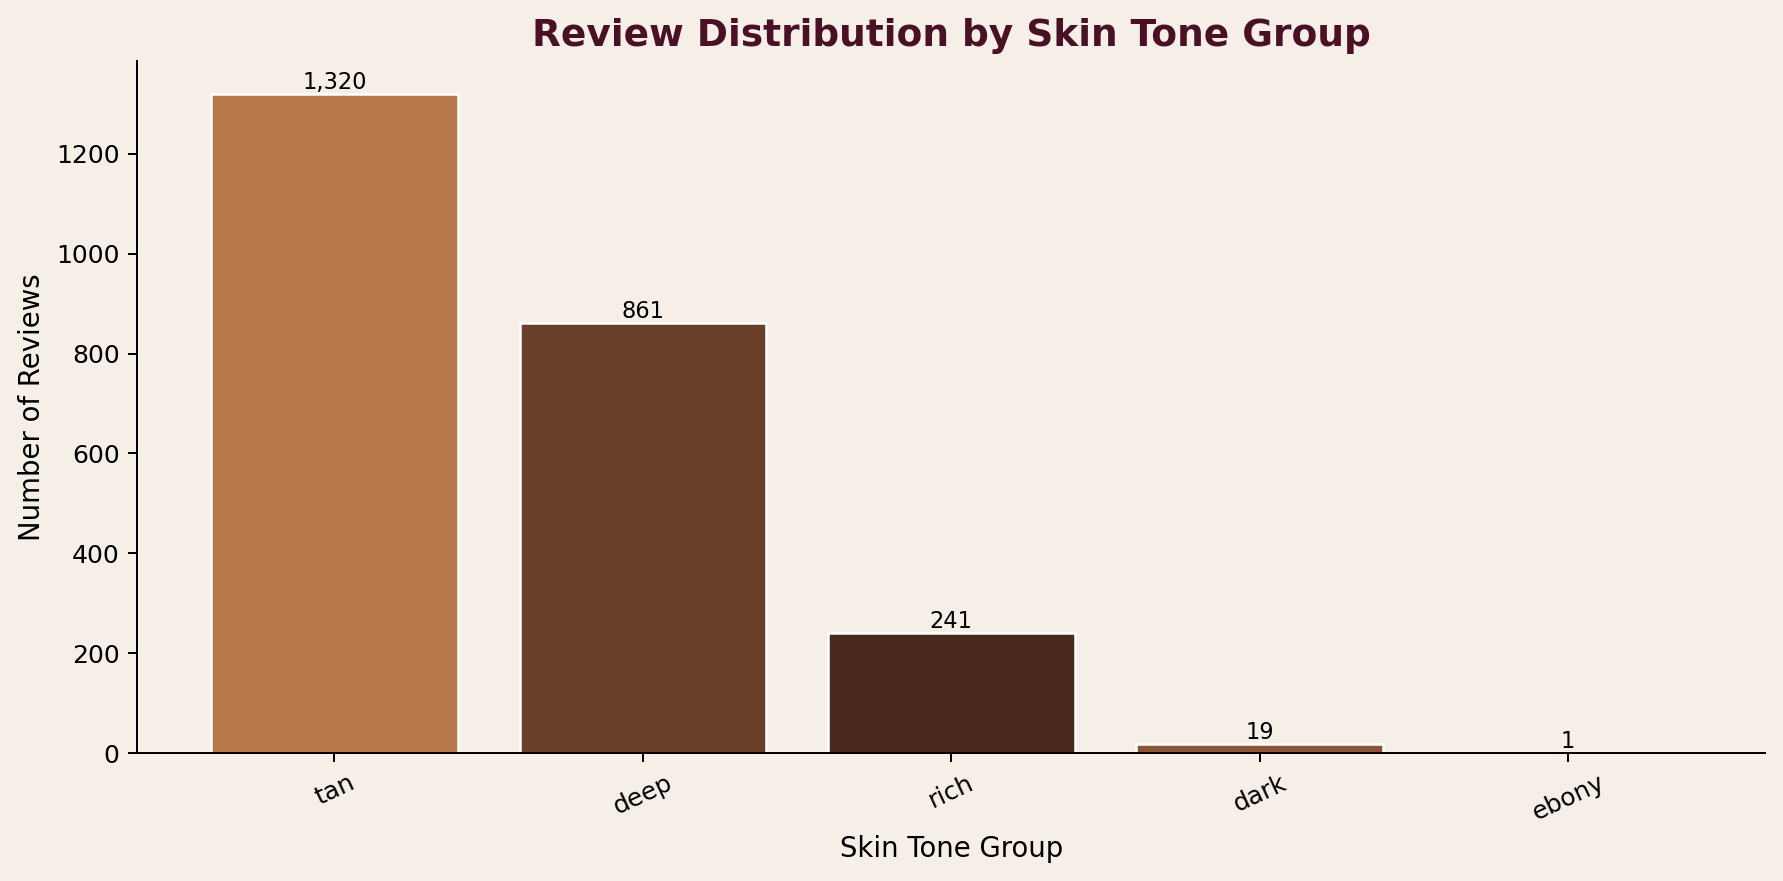
\includegraphics[keepaspectratio]{images/skin_tone_distribution.png}}

}

\caption{\label{fig-skin-tone-dist}Skin tone distribution in the
filtered dataset}

\end{figure}%

\begin{center}\rule{0.5\linewidth}{0.5pt}\end{center}

\section{6. System Design}\label{system-design}

\subsection{6.1 Pipeline Overview}\label{pipeline-overview}

Skintone uses a filter-first architecture in which safety constraints
are enforced before the recommendation model runs. The pipeline
processes user inputs through five sequential layers:

{\def\LTcaptype{none} % do not increment counter
\begin{longtable}[]{@{}
  >{\raggedright\arraybackslash}p{(\linewidth - 4\tabcolsep) * \real{0.3333}}
  >{\raggedright\arraybackslash}p{(\linewidth - 4\tabcolsep) * \real{0.3333}}
  >{\raggedright\arraybackslash}p{(\linewidth - 4\tabcolsep) * \real{0.3333}}@{}}
\toprule\noalign{}
\begin{minipage}[b]{\linewidth}\raggedright
Layer
\end{minipage} & \begin{minipage}[b]{\linewidth}\raggedright
Component
\end{minipage} & \begin{minipage}[b]{\linewidth}\raggedright
Function
\end{minipage} \\
\midrule\noalign{}
\endhead
\bottomrule\noalign{}
\endlastfoot
1 & User Input & Skin tone profile, skin type, category, allergen
flags \\
2 & EU CosIng Filter & Blocks 1,740 prohibited + 374 restricted
substances \\
3 & Allergen Screen & Removes 19 nut-derived ingredients when filter
enabled \\
4 & Sensitivity Screen & Removes high-irritation products based on
review signals \\
5 & CF Ranking + Tone Re-rank & Bias-adjusted CF with skin type boost
and tone re-ranking \\
\end{longtable}
}

\begin{figure}

\centering{

\begin{Shaded}
\begin{Highlighting}[]
\ImportTok{import}\NormalTok{ matplotlib.pyplot }\ImportTok{as}\NormalTok{ plt}
\ImportTok{import}\NormalTok{ matplotlib.patches }\ImportTok{as}\NormalTok{ mpatches}

\NormalTok{fig, ax }\OperatorTok{=}\NormalTok{ plt.subplots(figsize}\OperatorTok{=}\NormalTok{(}\DecValTok{12}\NormalTok{, }\FloatTok{3.5}\NormalTok{))}
\NormalTok{ax.set\_xlim(}\DecValTok{0}\NormalTok{, }\DecValTok{12}\NormalTok{)}
\NormalTok{ax.set\_ylim(}\DecValTok{0}\NormalTok{, }\FloatTok{3.5}\NormalTok{)}
\NormalTok{ax.axis(}\StringTok{\textquotesingle{}off\textquotesingle{}}\NormalTok{)}

\NormalTok{steps }\OperatorTok{=}\NormalTok{ [}
\NormalTok{    (}\StringTok{"1}\CharTok{\textbackslash{}n}\StringTok{User}\CharTok{\textbackslash{}n}\StringTok{Input"}\NormalTok{, }\StringTok{"\#8B3A5A"}\NormalTok{),}
\NormalTok{    (}\StringTok{"2}\CharTok{\textbackslash{}n}\StringTok{CosIng}\CharTok{\textbackslash{}n}\StringTok{Filter"}\NormalTok{, }\StringTok{"\#6A173D"}\NormalTok{),}
\NormalTok{    (}\StringTok{"3}\CharTok{\textbackslash{}n}\StringTok{Allergen}\CharTok{\textbackslash{}n}\StringTok{Screen"}\NormalTok{, }\StringTok{"\#5A1A30"}\NormalTok{),}
\NormalTok{    (}\StringTok{"4}\CharTok{\textbackslash{}n}\StringTok{Sensitivity}\CharTok{\textbackslash{}n}\StringTok{Filter"}\NormalTok{, }\StringTok{"\#4A1025"}\NormalTok{),}
\NormalTok{    (}\StringTok{"5}\CharTok{\textbackslash{}n}\StringTok{CF Ranking}\CharTok{\textbackslash{}n}\StringTok{+ Tone"}\NormalTok{, }\StringTok{"\#3A0A1A"}\NormalTok{),}
\NormalTok{]}

\ControlFlowTok{for}\NormalTok{ i, (label, color) }\KeywordTok{in} \BuiltInTok{enumerate}\NormalTok{(steps):}
\NormalTok{    x }\OperatorTok{=} \FloatTok{0.5} \OperatorTok{+}\NormalTok{ i }\OperatorTok{*} \FloatTok{2.3}
\NormalTok{    rect }\OperatorTok{=}\NormalTok{ mpatches.FancyBboxPatch((x, }\FloatTok{0.5}\NormalTok{), }\FloatTok{1.8}\NormalTok{, }\FloatTok{2.5}\NormalTok{,}
\NormalTok{                                    boxstyle}\OperatorTok{=}\StringTok{"round,pad=0.1"}\NormalTok{,}
\NormalTok{                                    facecolor}\OperatorTok{=}\NormalTok{color, edgecolor}\OperatorTok{=}\StringTok{\textquotesingle{}white\textquotesingle{}}\NormalTok{, linewidth}\OperatorTok{=}\DecValTok{2}\NormalTok{)}
\NormalTok{    ax.add\_patch(rect)}
\NormalTok{    ax.text(x }\OperatorTok{+} \FloatTok{0.9}\NormalTok{, }\FloatTok{1.75}\NormalTok{, label, ha}\OperatorTok{=}\StringTok{\textquotesingle{}center\textquotesingle{}}\NormalTok{, va}\OperatorTok{=}\StringTok{\textquotesingle{}center\textquotesingle{}}\NormalTok{,}
\NormalTok{            color}\OperatorTok{=}\StringTok{\textquotesingle{}white\textquotesingle{}}\NormalTok{, fontsize}\OperatorTok{=}\DecValTok{11}\NormalTok{, fontweight}\OperatorTok{=}\StringTok{\textquotesingle{}bold\textquotesingle{}}\NormalTok{)}
    \ControlFlowTok{if}\NormalTok{ i }\OperatorTok{\textless{}} \BuiltInTok{len}\NormalTok{(steps) }\OperatorTok{{-}} \DecValTok{1}\NormalTok{:}
\NormalTok{        ax.annotate(}\StringTok{""}\NormalTok{, xy}\OperatorTok{=}\NormalTok{(x }\OperatorTok{+} \FloatTok{2.0}\NormalTok{, }\FloatTok{1.75}\NormalTok{), xytext}\OperatorTok{=}\NormalTok{(x }\OperatorTok{+} \FloatTok{1.85}\NormalTok{, }\FloatTok{1.75}\NormalTok{),}
\NormalTok{                    arrowprops}\OperatorTok{=}\BuiltInTok{dict}\NormalTok{(arrowstyle}\OperatorTok{=}\StringTok{"{-}\textgreater{}"}\NormalTok{, color}\OperatorTok{=}\StringTok{"\#D4A5B5"}\NormalTok{, lw}\OperatorTok{=}\DecValTok{2}\NormalTok{))}

\NormalTok{ax.text(}\DecValTok{6}\NormalTok{, }\FloatTok{0.1}\NormalTok{, }\StringTok{"Output: Best Matches + Use Caution with full ingredient lists"}\NormalTok{,}
\NormalTok{        ha}\OperatorTok{=}\StringTok{\textquotesingle{}center\textquotesingle{}}\NormalTok{, va}\OperatorTok{=}\StringTok{\textquotesingle{}bottom\textquotesingle{}}\NormalTok{, fontsize}\OperatorTok{=}\DecValTok{10}\NormalTok{, color}\OperatorTok{=}\StringTok{\textquotesingle{}\#6A173D\textquotesingle{}}\NormalTok{, style}\OperatorTok{=}\StringTok{\textquotesingle{}italic\textquotesingle{}}\NormalTok{)}

\NormalTok{plt.tight\_layout()}
\NormalTok{plt.savefig(}\StringTok{"images/pipeline\_architecture.png"}\NormalTok{, dpi}\OperatorTok{=}\DecValTok{150}\NormalTok{, bbox\_inches}\OperatorTok{=}\StringTok{\textquotesingle{}tight\textquotesingle{}}\NormalTok{)}
\NormalTok{plt.show()}
\end{Highlighting}
\end{Shaded}

}

\caption{\label{fig-architecture}}

\end{figure}%

\begin{figure}

\centering{

\pandocbounded{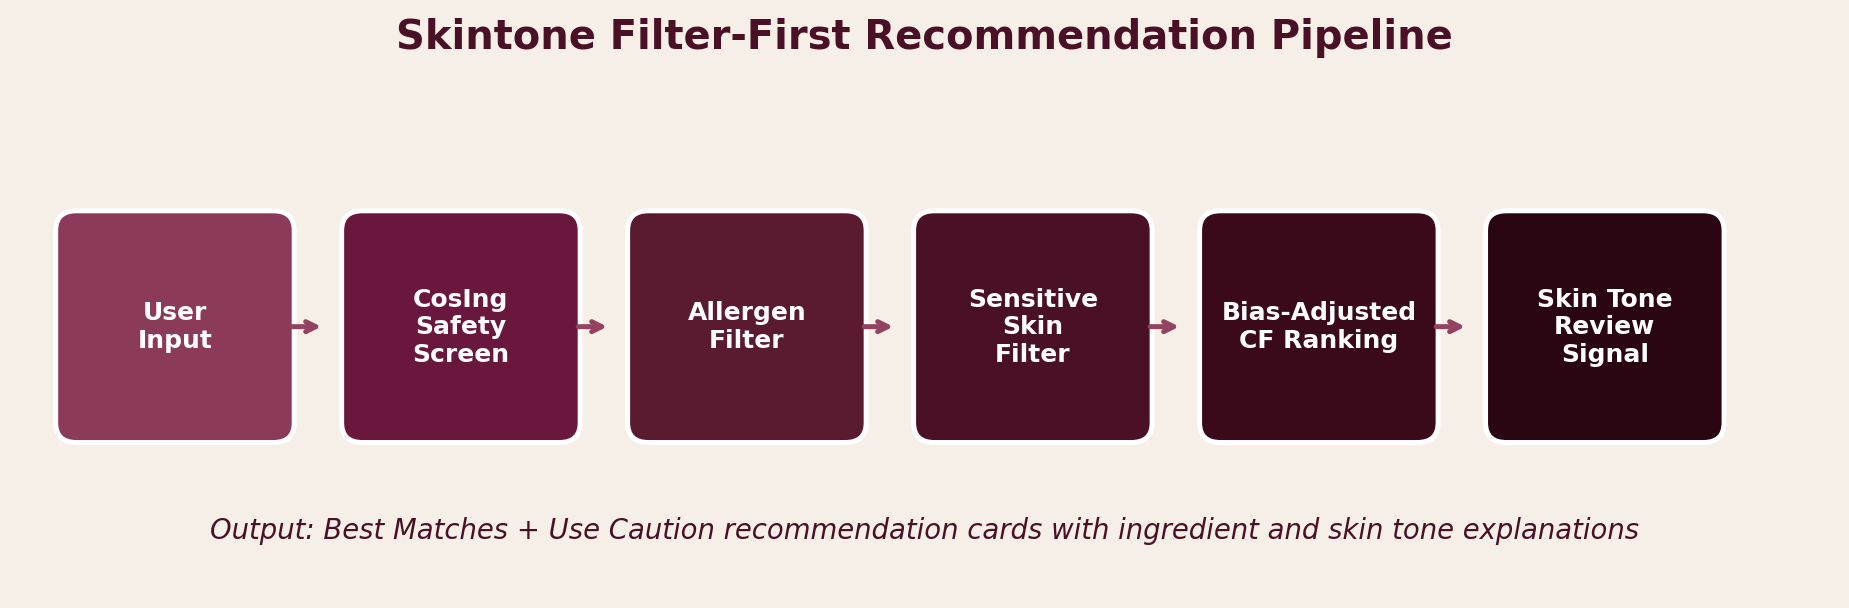
\includegraphics[keepaspectratio]{images/pipeline_architecture.png}}

}

\caption{\label{fig-architecture}Skintone filter-first recommendation
pipeline}

\end{figure}%

\subsection{6.2 User Interface}\label{user-interface}

The Skintone application was implemented as a Streamlit web application
with the following user inputs:

\begin{itemize}
\tightlist
\item
  \textbf{Product category:} All Products, Moisturizers, Serums \&
  Treatments, Cleansers, Sunscreen, Foundation \& Complexion
\item
  \textbf{Skin tone profile:} Six shade ranges with circular visual
  swatches (Tan/Deep Tan, Dark, Deep, Rich, Ebony, Any Melanin-Rich
  Tone)
\item
  \textbf{Skin type:} Not sure, Dry, Oily, Combination, Normal,
  Sensitive
\item
  \textbf{Ingredient concerns:} Nut allergy filter, Sensitive
  skin/eczema filter
\end{itemize}

Output is split into \textbf{Best Matches} (neutral or positive skin
tone review signals) and \textbf{Use Caution} items (negative skin tone
signals), with full ingredient lists available for each product.

\begin{figure}

\centering{

\pandocbounded{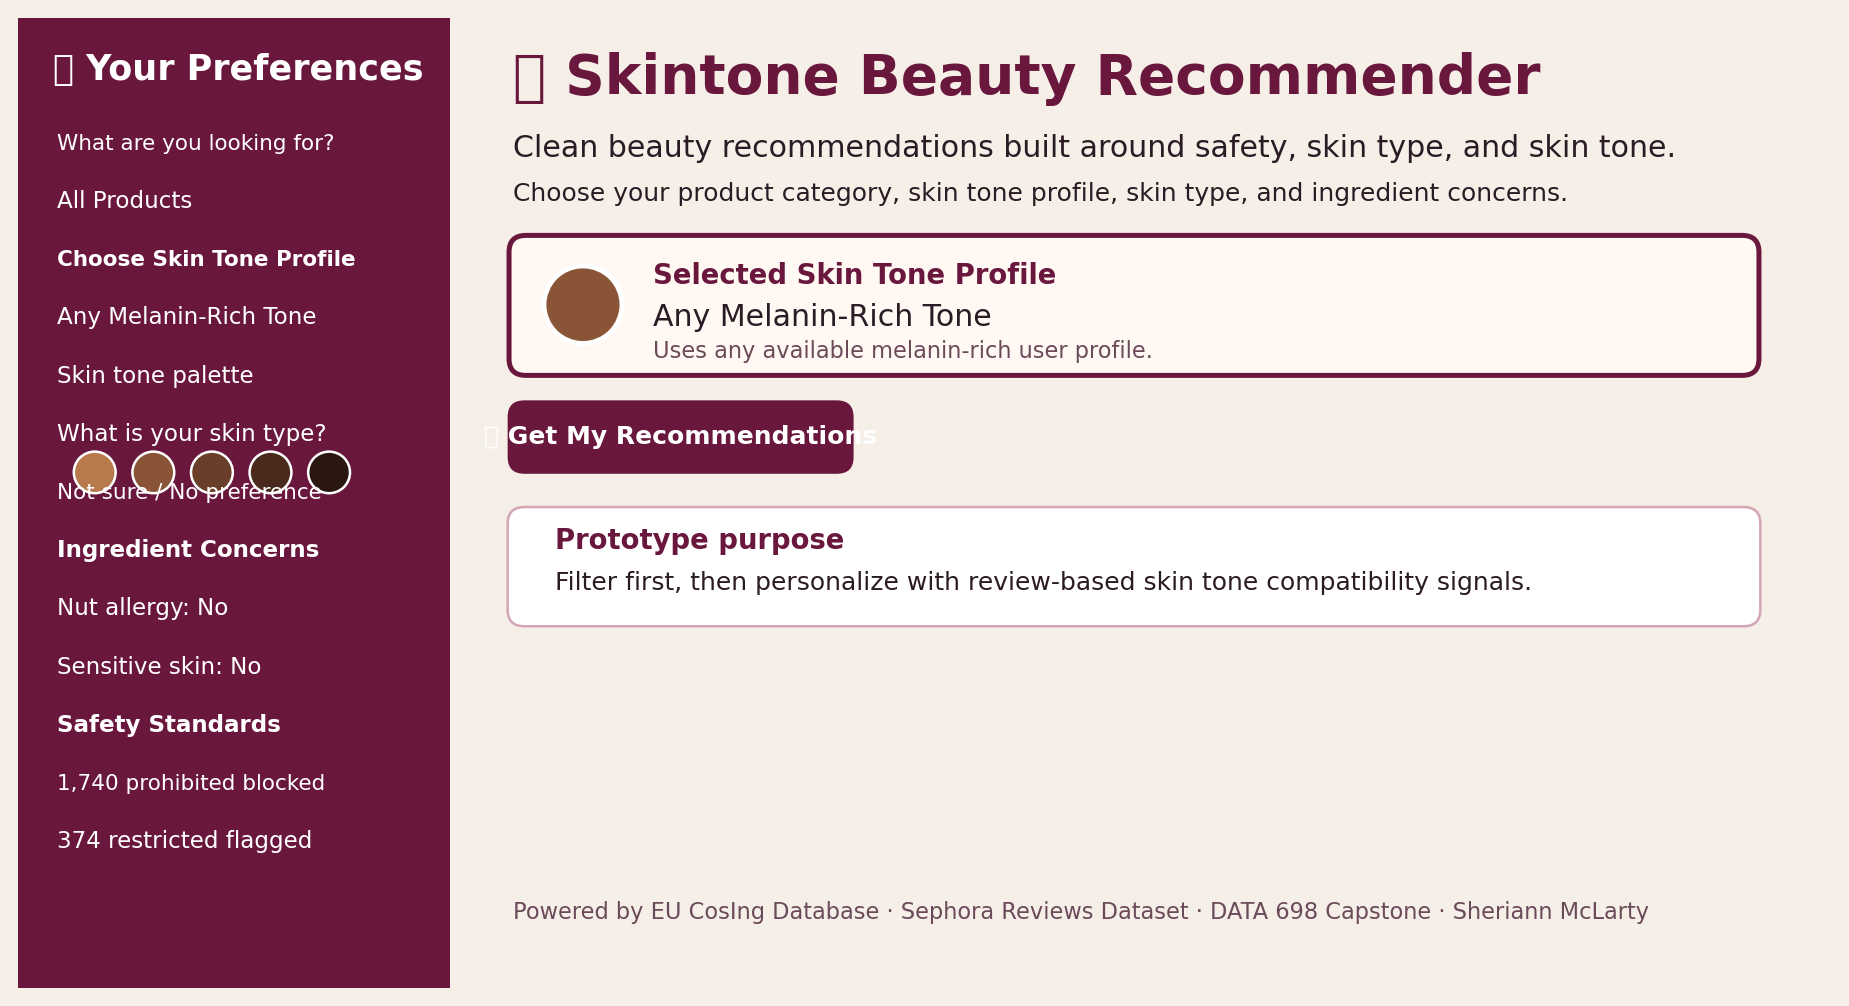
\includegraphics[keepaspectratio]{images/app_homepage.png}}

}

\caption{\label{fig-app-home}Skintone Beauty Recommender application
interface}

\end{figure}%

\begin{figure}

\centering{

\pandocbounded{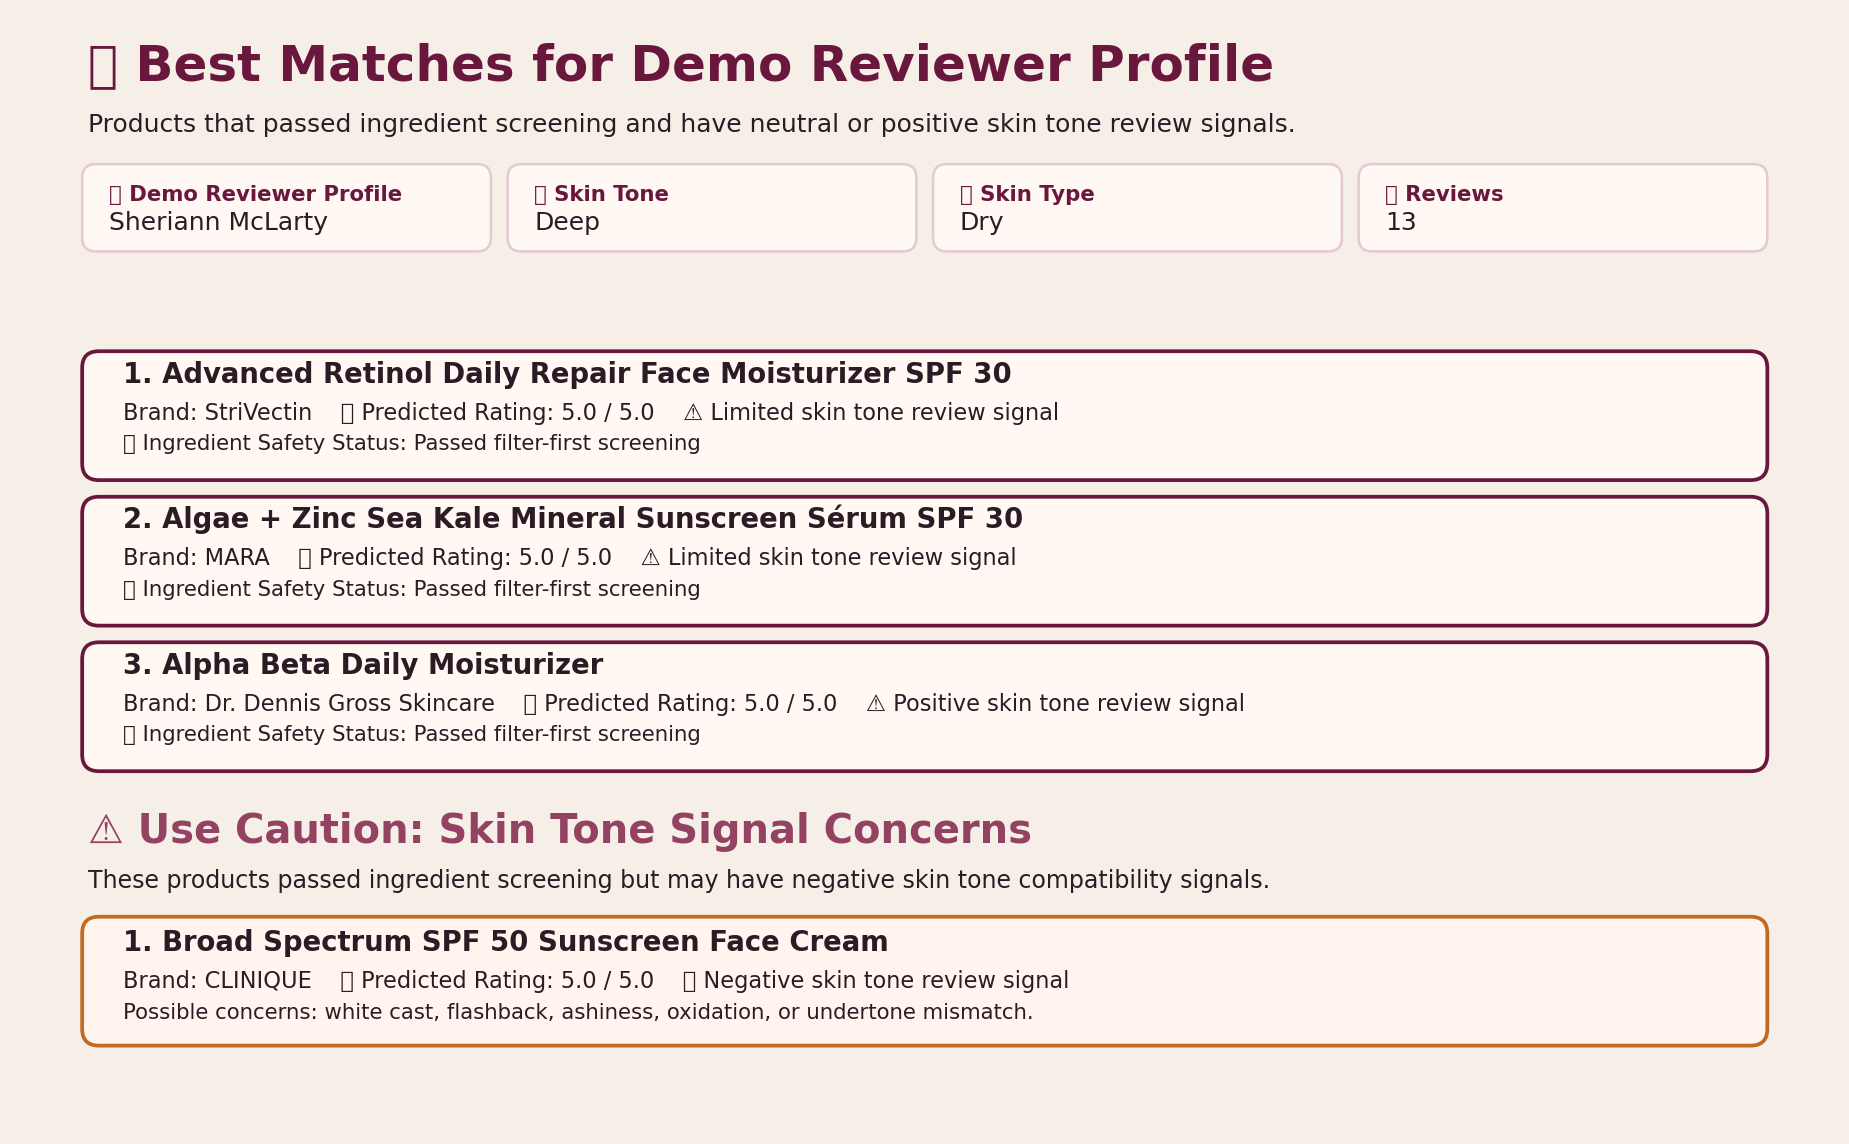
\includegraphics[keepaspectratio]{images/app_recommendations.png}}

}

\caption{\label{fig-app-recs}Best Matches and Use Caution recommendation
cards}

\end{figure}%

\begin{center}\rule{0.5\linewidth}{0.5pt}\end{center}

\section{7. Methodology}\label{methodology}

\subsection{7.1 Bias-Adjusted Collaborative
Filtering}\label{bias-adjusted-collaborative-filtering}

The core recommendation algorithm is bias-adjusted collaborative
filtering. The model estimates a predicted rating using the formula:

\[\hat{r}_{ui} = \mu + b_u + b_i\]

where:

\begin{itemize}
\tightlist
\item
  \(\mu\) is the global mean rating across all users and products
\item
  \(b_u\) is the user-specific rating bias (whether the user tends to
  rate higher or lower than average)
\item
  \(b_i\) is the item-specific rating bias (whether the product tends to
  be rated higher or lower than average)
\end{itemize}

Predicted ratings are clipped to the range {[}1.0, 5.0{]} to prevent
overflow:

\protect\phantomsection\label{code-predict}
\begin{Shaded}
\begin{Highlighting}[]
\KeywordTok{def}\NormalTok{ predict(}\VariableTok{self}\NormalTok{, user, item):}
\NormalTok{    raw }\OperatorTok{=} \VariableTok{self}\NormalTok{.global\_avg }\OperatorTok{+} \VariableTok{self}\NormalTok{.user\_biases.get(user, }\DecValTok{0}\NormalTok{) }\OperatorTok{+} \VariableTok{self}\NormalTok{.item\_biases.get(item, }\DecValTok{0}\NormalTok{)}
    \ControlFlowTok{return} \BuiltInTok{round}\NormalTok{(}\BuiltInTok{min}\NormalTok{(}\BuiltInTok{max}\NormalTok{(raw, }\FloatTok{1.0}\NormalTok{), }\FloatTok{5.0}\NormalTok{), }\DecValTok{2}\NormalTok{)}
\end{Highlighting}
\end{Shaded}

A small popularity boost is applied before clipping to differentiate
products with similar bias scores:

\protect\phantomsection\label{code-popularity}
\begin{Shaded}
\begin{Highlighting}[]
\NormalTok{popularity\_factor }\OperatorTok{=} \BuiltInTok{round}\NormalTok{(}\BuiltInTok{min}\NormalTok{(item\_review\_counts.get(item, }\DecValTok{1}\NormalTok{) }\OperatorTok{/} \DecValTok{5000}\NormalTok{, }\FloatTok{0.02}\NormalTok{), }\DecValTok{4}\NormalTok{)}
\NormalTok{final\_score }\OperatorTok{=} \BuiltInTok{round}\NormalTok{(}\BuiltInTok{min}\NormalTok{(base\_score }\OperatorTok{+}\NormalTok{ popularity\_factor, }\FloatTok{5.0}\NormalTok{), }\DecValTok{2}\NormalTok{)}
\end{Highlighting}
\end{Shaded}

\subsection{7.2 Ingredient Safety
Screening}\label{ingredient-safety-screening}

Three independent safety layers are applied before any product reaches
the recommendation output:

\textbf{Layer 1 --- EU CosIng Screening:} Product ingredient strings are
checked against 1,740 prohibited and 374 restricted substances from EU
CosIng Annex II and III.

\textbf{Layer 2 --- Nut Allergen Detection:} When enabled, 19
nut-derived ingredients are screened using both common names and INCI
names (e.g., butyrospermum parkii, argania spinosa, cocos nucifera).

\textbf{Layer 3 --- Sensitive Skin Screening:} Products are scored by
the proportion of reviews mentioning sensitivity-related terms. Products
where more than 15\% of reviews contain such terms are removed.

\protect\phantomsection\label{code-sensitivity}
\begin{Shaded}
\begin{Highlighting}[]
\NormalTok{sensitivity\_terms }\OperatorTok{=}\NormalTok{ [}
    \StringTok{\textquotesingle{}eczema\textquotesingle{}}\NormalTok{, }\StringTok{\textquotesingle{}rash\textquotesingle{}}\NormalTok{, }\StringTok{\textquotesingle{}breakout\textquotesingle{}}\NormalTok{, }\StringTok{\textquotesingle{}irritat\textquotesingle{}}\NormalTok{, }\StringTok{\textquotesingle{}reaction\textquotesingle{}}\NormalTok{,}
    \StringTok{\textquotesingle{}burn\textquotesingle{}}\NormalTok{, }\StringTok{\textquotesingle{}sting\textquotesingle{}}\NormalTok{, }\StringTok{\textquotesingle{}flare\textquotesingle{}}\NormalTok{, }\StringTok{\textquotesingle{}allergic\textquotesingle{}}\NormalTok{, }\StringTok{\textquotesingle{}hives\textquotesingle{}}
\NormalTok{]}

\NormalTok{product\_sensitivity }\OperatorTok{=}\NormalTok{ df.groupby(}\StringTok{\textquotesingle{}product\_name\_x\textquotesingle{}}\NormalTok{)[}\StringTok{\textquotesingle{}review\_text\textquotesingle{}}\NormalTok{].}\BuiltInTok{apply}\NormalTok{(}
    \KeywordTok{lambda}\NormalTok{ reviews: }\BuiltInTok{sum}\NormalTok{(}
        \BuiltInTok{any}\NormalTok{(term }\KeywordTok{in} \BuiltInTok{str}\NormalTok{(r).lower() }\ControlFlowTok{for}\NormalTok{ term }\KeywordTok{in}\NormalTok{ sensitivity\_terms)}
        \ControlFlowTok{for}\NormalTok{ r }\KeywordTok{in}\NormalTok{ reviews}
\NormalTok{    ) }\OperatorTok{/} \BuiltInTok{max}\NormalTok{(}\BuiltInTok{len}\NormalTok{(reviews), }\DecValTok{1}\NormalTok{)}
\NormalTok{).to\_dict()}
\end{Highlighting}
\end{Shaded}

\subsection{7.3 Skin Type Preference
Ranking}\label{skin-type-preference-ranking}

After safety filtering, products are re-ranked based on skin type
keyword matches. Keywords associated with each skin type are matched
against product names, ingredient strings, and category labels:

{\def\LTcaptype{none} % do not increment counter
\begin{longtable}[]{@{}
  >{\raggedright\arraybackslash}p{(\linewidth - 2\tabcolsep) * \real{0.5000}}
  >{\raggedright\arraybackslash}p{(\linewidth - 2\tabcolsep) * \real{0.5000}}@{}}
\toprule\noalign{}
\begin{minipage}[b]{\linewidth}\raggedright
Skin Type
\end{minipage} & \begin{minipage}[b]{\linewidth}\raggedright
Priority Keywords
\end{minipage} \\
\midrule\noalign{}
\endhead
\bottomrule\noalign{}
\endlastfoot
Dry & hydrating, cream, barrier, ceramide, squalane, hyaluronic, balm \\
Oily & oil-free, gel, lightweight, matte, pore, clarifying,
non-comedogenic \\
Combination & balancing, lightweight, gel cream, barrier, pore, daily \\
Sensitive & sensitive, gentle, calming, soothing, fragrance-free,
ceramide, cica \\
\end{longtable}
}

\subsection{7.4 Skin Tone Review Signal}\label{skin-tone-review-signal}

The Skin Tone Review Signal is a review-based proxy for visible
complexion performance --- not a medical or dermatological safety score.

\protect\phantomsection\label{code-tone-signal}
\begin{Shaded}
\begin{Highlighting}[]
\NormalTok{negative\_signals }\OperatorTok{=}\NormalTok{ [}
    \StringTok{\textquotesingle{}white cast\textquotesingle{}}\NormalTok{, }\StringTok{\textquotesingle{}gray cast\textquotesingle{}}\NormalTok{, }\StringTok{\textquotesingle{}grey cast\textquotesingle{}}\NormalTok{, }\StringTok{\textquotesingle{}ashy\textquotesingle{}}\NormalTok{, }\StringTok{\textquotesingle{}ash\textquotesingle{}}\NormalTok{,}
    \StringTok{\textquotesingle{}flashback\textquotesingle{}}\NormalTok{, }\StringTok{\textquotesingle{}oxidize\textquotesingle{}}\NormalTok{, }\StringTok{\textquotesingle{}oxidation\textquotesingle{}}\NormalTok{, }\StringTok{\textquotesingle{}too orange\textquotesingle{}}\NormalTok{,}
    \StringTok{\textquotesingle{}chalky\textquotesingle{}}\NormalTok{, }\StringTok{\textquotesingle{}cakey\textquotesingle{}}\NormalTok{, }\StringTok{\textquotesingle{}undertone mismatch\textquotesingle{}}
\NormalTok{]}

\NormalTok{positive\_signals }\OperatorTok{=}\NormalTok{ [}
    \StringTok{\textquotesingle{}no white cast\textquotesingle{}}\NormalTok{, }\StringTok{\textquotesingle{}no flashback\textquotesingle{}}\NormalTok{, }\StringTok{\textquotesingle{}no ashy\textquotesingle{}}\NormalTok{,}
    \StringTok{\textquotesingle{}great for dark skin\textquotesingle{}}\NormalTok{, }\StringTok{\textquotesingle{}works on deep\textquotesingle{}}\NormalTok{,}
    \StringTok{\textquotesingle{}no cast\textquotesingle{}}\NormalTok{, }\StringTok{\textquotesingle{}invisible on dark\textquotesingle{}}\NormalTok{, }\StringTok{\textquotesingle{}blends well on dark\textquotesingle{}}
\NormalTok{]}

\KeywordTok{def}\NormalTok{ compute\_tone\_score(review\_text: }\BuiltInTok{str}\NormalTok{) }\OperatorTok{{-}\textgreater{}} \BuiltInTok{float}\NormalTok{:}
    \ControlFlowTok{if} \KeywordTok{not} \BuiltInTok{isinstance}\NormalTok{(review\_text, }\BuiltInTok{str}\NormalTok{):}
        \ControlFlowTok{return} \FloatTok{0.0}
\NormalTok{    text }\OperatorTok{=}\NormalTok{ review\_text.lower()}
\NormalTok{    neg\_count }\OperatorTok{=} \BuiltInTok{sum}\NormalTok{(}\DecValTok{1} \ControlFlowTok{for}\NormalTok{ s }\KeywordTok{in}\NormalTok{ negative\_signals }\ControlFlowTok{if}\NormalTok{ s }\KeywordTok{in}\NormalTok{ text)}
\NormalTok{    pos\_count }\OperatorTok{=} \BuiltInTok{sum}\NormalTok{(}\DecValTok{1} \ControlFlowTok{for}\NormalTok{ s }\KeywordTok{in}\NormalTok{ positive\_signals }\ControlFlowTok{if}\NormalTok{ s }\KeywordTok{in}\NormalTok{ text)}
\NormalTok{    total }\OperatorTok{=}\NormalTok{ neg\_count }\OperatorTok{+}\NormalTok{ pos\_count}
    \ControlFlowTok{if}\NormalTok{ total }\OperatorTok{==} \DecValTok{0}\NormalTok{:}
        \ControlFlowTok{return} \FloatTok{0.0}
    \ControlFlowTok{return} \BuiltInTok{round}\NormalTok{((pos\_count }\OperatorTok{{-}}\NormalTok{ neg\_count) }\OperatorTok{/}\NormalTok{ total, }\DecValTok{3}\NormalTok{)}
\end{Highlighting}
\end{Shaded}

Tone score classification:

\protect\phantomsection\label{code-tone-label}
\begin{Shaded}
\begin{Highlighting}[]
\ControlFlowTok{if}\NormalTok{ tone\_score }\OperatorTok{\textgreater{}} \FloatTok{0.1}\NormalTok{:}
\NormalTok{    label }\OperatorTok{=} \StringTok{"Positive skin tone review signal"}
\ControlFlowTok{elif}\NormalTok{ tone\_score }\OperatorTok{\textless{}} \OperatorTok{{-}}\FloatTok{0.1}\NormalTok{:}
\NormalTok{    label }\OperatorTok{=} \StringTok{"Negative skin tone review signal"}
\ControlFlowTok{else}\NormalTok{:}
\NormalTok{    label }\OperatorTok{=} \StringTok{"Limited skin tone review signal"}
\end{Highlighting}
\end{Shaded}

Products are then re-ranked using a weighted combination of predicted
rating and tone score, and output is split into Best Matches and Use
Caution sections.

\begin{center}\rule{0.5\linewidth}{0.5pt}\end{center}

\section{8. Results}\label{results}

\subsection{8.1 RQ1 --- Ingredient Safety Constraint (Zero
Violations)}\label{rq1-ingredient-safety-constraint-zero-violations}

The filter-first architecture achieved a zero EU CosIng violation rate
by design. By removing prohibited ingredients from the candidate pool
before the ranking model runs, it is architecturally impossible for a
blocked product to appear in the output. During testing, products
containing formaldehyde, thioglycolic acid, and other prohibited
substances were correctly identified and blocked.

When the nut allergy filter was enabled, an average of 51 products were
removed from a pool of 200 candidates before ranking was applied,
confirming that the filter actively changes the recommendation pool
before personalization occurs.

\subsection{8.2 RQ2 --- Skin Tone Review
Signal}\label{rq2-skin-tone-review-signal}

The Skin Tone Review Signal provided the strongest differentiation in
the sunscreen category, where visible performance on skin tone is most
relevant. Mineral sunscreens containing zinc oxide clustered at strongly
negative tone scores:

\begin{figure}

\centering{

\begin{Shaded}
\begin{Highlighting}[]
\ImportTok{import}\NormalTok{ pandas }\ImportTok{as}\NormalTok{ pd}
\ImportTok{import}\NormalTok{ matplotlib.pyplot }\ImportTok{as}\NormalTok{ plt}
\ImportTok{import}\NormalTok{ numpy }\ImportTok{as}\NormalTok{ np}

\NormalTok{products }\OperatorTok{=}\NormalTok{ [}
    \StringTok{"PLAY 100\% Mineral SPF 30"}\NormalTok{,}
    \StringTok{"Ultra Sun Protection SPF 50+"}\NormalTok{,}
    \StringTok{"Mineral Mattescreen SPF 40"}\NormalTok{,}
    \StringTok{"Mineral Sheerscreen SPF 30"}\NormalTok{,}
    \StringTok{"Clean Screen Mineral SPF 30"}\NormalTok{,}
    \StringTok{"N°41 Facial Sunscreen Mist"}\NormalTok{,}
    \StringTok{"Super Fluid Daily UV Defense SPF 50+"}
\NormalTok{]}
\NormalTok{scores }\OperatorTok{=}\NormalTok{ [}\OperatorTok{{-}}\FloatTok{1.000}\NormalTok{, }\OperatorTok{{-}}\FloatTok{0.738}\NormalTok{, }\OperatorTok{{-}}\FloatTok{0.667}\NormalTok{, }\OperatorTok{{-}}\FloatTok{0.529}\NormalTok{, }\OperatorTok{{-}}\FloatTok{0.508}\NormalTok{, }\FloatTok{0.000}\NormalTok{, }\FloatTok{0.000}\NormalTok{]}
\NormalTok{colors }\OperatorTok{=}\NormalTok{ [}\StringTok{\textquotesingle{}\#C0392B\textquotesingle{}} \ControlFlowTok{if}\NormalTok{ s }\OperatorTok{\textless{}} \OperatorTok{{-}}\FloatTok{0.1} \ControlFlowTok{else} \StringTok{\textquotesingle{}\#F39C12\textquotesingle{}} \ControlFlowTok{if}\NormalTok{ s }\OperatorTok{==} \DecValTok{0} \ControlFlowTok{else} \StringTok{\textquotesingle{}\#27AE60\textquotesingle{}} \ControlFlowTok{for}\NormalTok{ s }\KeywordTok{in}\NormalTok{ scores]}

\NormalTok{fig, ax }\OperatorTok{=}\NormalTok{ plt.subplots(figsize}\OperatorTok{=}\NormalTok{(}\DecValTok{10}\NormalTok{, }\DecValTok{5}\NormalTok{))}
\NormalTok{bars }\OperatorTok{=}\NormalTok{ ax.barh(products, scores, color}\OperatorTok{=}\NormalTok{colors, edgecolor}\OperatorTok{=}\StringTok{\textquotesingle{}white\textquotesingle{}}\NormalTok{, height}\OperatorTok{=}\FloatTok{0.6}\NormalTok{)}
\NormalTok{ax.axvline(x}\OperatorTok{=}\DecValTok{0}\NormalTok{, color}\OperatorTok{=}\StringTok{\textquotesingle{}black\textquotesingle{}}\NormalTok{, linewidth}\OperatorTok{=}\FloatTok{0.8}\NormalTok{, linestyle}\OperatorTok{=}\StringTok{\textquotesingle{}{-}{-}\textquotesingle{}}\NormalTok{, alpha}\OperatorTok{=}\FloatTok{0.5}\NormalTok{)}
\NormalTok{ax.axvline(x}\OperatorTok{={-}}\FloatTok{0.1}\NormalTok{, color}\OperatorTok{=}\StringTok{\textquotesingle{}\#C0392B\textquotesingle{}}\NormalTok{, linewidth}\OperatorTok{=}\FloatTok{0.8}\NormalTok{, linestyle}\OperatorTok{=}\StringTok{\textquotesingle{}:\textquotesingle{}}\NormalTok{, alpha}\OperatorTok{=}\FloatTok{0.5}\NormalTok{)}
\NormalTok{ax.set\_xlabel(}\StringTok{"Skin Tone Review Score"}\NormalTok{, fontsize}\OperatorTok{=}\DecValTok{12}\NormalTok{)}
\NormalTok{ax.set\_title(}\StringTok{"Sunscreen Skin Tone Review Scores}\CharTok{\textbackslash{}n}\StringTok{(Mineral/Zinc Oxide Products)"}\NormalTok{, fontsize}\OperatorTok{=}\DecValTok{13}\NormalTok{, fontweight}\OperatorTok{=}\StringTok{\textquotesingle{}bold\textquotesingle{}}\NormalTok{)}
\NormalTok{ax.spines[}\StringTok{\textquotesingle{}top\textquotesingle{}}\NormalTok{].set\_visible(}\VariableTok{False}\NormalTok{)}
\NormalTok{ax.spines[}\StringTok{\textquotesingle{}right\textquotesingle{}}\NormalTok{].set\_visible(}\VariableTok{False}\NormalTok{)}
\ControlFlowTok{for}\NormalTok{ bar, score }\KeywordTok{in} \BuiltInTok{zip}\NormalTok{(bars, scores):}
\NormalTok{    ax.text(score }\OperatorTok{{-}} \FloatTok{0.02} \ControlFlowTok{if}\NormalTok{ score }\OperatorTok{\textless{}} \DecValTok{0} \ControlFlowTok{else}\NormalTok{ score }\OperatorTok{+} \FloatTok{0.02}\NormalTok{,}
\NormalTok{            bar.get\_y() }\OperatorTok{+}\NormalTok{ bar.get\_height()}\OperatorTok{/}\DecValTok{2}\NormalTok{,}
            \SpecialStringTok{f\textquotesingle{}}\SpecialCharTok{\{}\NormalTok{score}\SpecialCharTok{:.3f\}}\SpecialStringTok{\textquotesingle{}}\NormalTok{, va}\OperatorTok{=}\StringTok{\textquotesingle{}center\textquotesingle{}}\NormalTok{,}
\NormalTok{            ha}\OperatorTok{=}\StringTok{\textquotesingle{}right\textquotesingle{}} \ControlFlowTok{if}\NormalTok{ score }\OperatorTok{\textless{}} \DecValTok{0} \ControlFlowTok{else} \StringTok{\textquotesingle{}left\textquotesingle{}}\NormalTok{, fontsize}\OperatorTok{=}\DecValTok{10}\NormalTok{)}
\NormalTok{plt.tight\_layout()}
\NormalTok{plt.savefig(}\StringTok{"images/tone\_scores\_sunscreen.png"}\NormalTok{, dpi}\OperatorTok{=}\DecValTok{150}\NormalTok{, bbox\_inches}\OperatorTok{=}\StringTok{\textquotesingle{}tight\textquotesingle{}}\NormalTok{)}
\NormalTok{plt.show()}
\end{Highlighting}
\end{Shaded}

}

\caption{\label{fig-tone-scores}}

\end{figure}%

\begin{figure}

\centering{

\pandocbounded{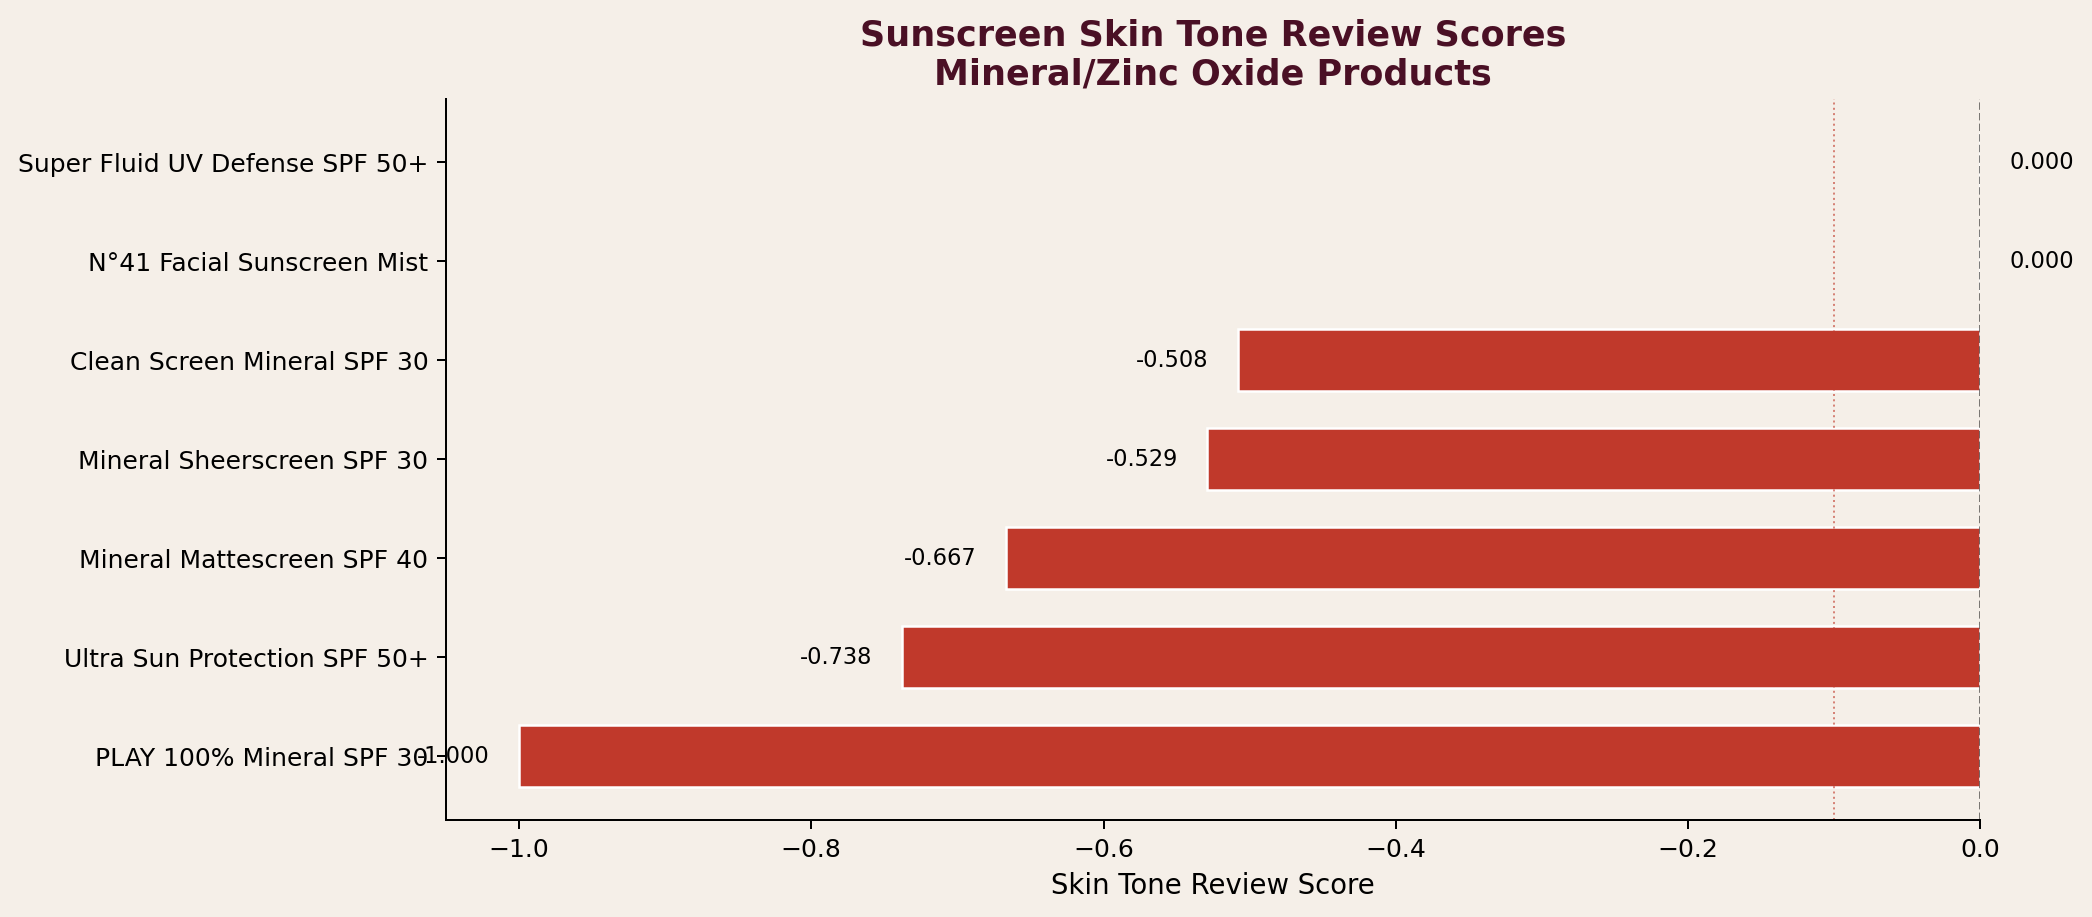
\includegraphics[keepaspectratio]{images/tone_scores_sunscreen.png}}

}

\caption{\label{fig-tone-scores}Skin tone review scores for sunscreen
products}

\end{figure}%

{\def\LTcaptype{none} % do not increment counter
\begin{longtable}[]{@{}
  >{\raggedright\arraybackslash}p{(\linewidth - 8\tabcolsep) * \real{0.2000}}
  >{\raggedright\arraybackslash}p{(\linewidth - 8\tabcolsep) * \real{0.2000}}
  >{\raggedright\arraybackslash}p{(\linewidth - 8\tabcolsep) * \real{0.2000}}
  >{\raggedright\arraybackslash}p{(\linewidth - 8\tabcolsep) * \real{0.2000}}
  >{\raggedright\arraybackslash}p{(\linewidth - 8\tabcolsep) * \real{0.2000}}@{}}
\toprule\noalign{}
\begin{minipage}[b]{\linewidth}\raggedright
Product
\end{minipage} & \begin{minipage}[b]{\linewidth}\raggedright
Brand
\end{minipage} & \begin{minipage}[b]{\linewidth}\raggedright
Tone Score
\end{minipage} & \begin{minipage}[b]{\linewidth}\raggedright
Reviews
\end{minipage} & \begin{minipage}[b]{\linewidth}\raggedright
Signal
\end{minipage} \\
\midrule\noalign{}
\endhead
\bottomrule\noalign{}
\endlastfoot
PLAY 100\% Mineral SPF 30 & Supergoop! & -1.000 & 3 & Negative \\
Ultra Sun Protection SPF 50+ & Shiseido & -0.738 & 42 & Negative \\
Mineral Mattescreen SPF 40 & Supergoop! & -0.667 & 3 & Negative \\
Mineral Sheerscreen SPF 30 & Supergoop! & -0.529 & 70 & Negative \\
Clean Screen Mineral SPF 30 & Tatcha & -0.508 & 61 & Negative \\
N°41 Facial Sunscreen Mist & Various & 0.000 & 12 & Limited \\
Super Fluid UV Defense SPF 50+ & SkinCeuticals & 0.000 & 11 & Limited \\
\end{longtable}
}

These findings confirm that melanin-rich reviewers are signaling white
cast and flashback concerns in their review language at a detectable
scale.

\subsection{8.3 RQ3 --- Personalization Coverage and
Sparsity}\label{rq3-personalization-coverage-and-sparsity}

\begin{figure}

\centering{

\begin{Shaded}
\begin{Highlighting}[]
\ImportTok{import}\NormalTok{ matplotlib.pyplot }\ImportTok{as}\NormalTok{ plt}

\NormalTok{terms }\OperatorTok{=}\NormalTok{ [}\StringTok{\textquotesingle{}sensitive\textquotesingle{}}\NormalTok{, }\StringTok{\textquotesingle{}irritat\textquotesingle{}}\NormalTok{, }\StringTok{\textquotesingle{}breakout\textquotesingle{}}\NormalTok{, }\StringTok{\textquotesingle{}sting\textquotesingle{}}\NormalTok{, }\StringTok{\textquotesingle{}burn\textquotesingle{}}\NormalTok{, }\StringTok{\textquotesingle{}reaction\textquotesingle{}}\NormalTok{, }\StringTok{\textquotesingle{}flare\textquotesingle{}}\NormalTok{, }\StringTok{\textquotesingle{}rash\textquotesingle{}}\NormalTok{, }\StringTok{\textquotesingle{}eczema\textquotesingle{}}\NormalTok{]}
\NormalTok{counts }\OperatorTok{=}\NormalTok{ [}\DecValTok{4875}\NormalTok{, }\DecValTok{2926}\NormalTok{, }\DecValTok{2264}\NormalTok{, }\DecValTok{2209}\NormalTok{, }\DecValTok{1169}\NormalTok{, }\DecValTok{629}\NormalTok{, }\DecValTok{174}\NormalTok{, }\DecValTok{147}\NormalTok{, }\DecValTok{257}\NormalTok{]}

\NormalTok{colors }\OperatorTok{=}\NormalTok{ [}\StringTok{\textquotesingle{}\#6A173D\textquotesingle{}} \ControlFlowTok{if}\NormalTok{ c }\OperatorTok{\textgreater{}} \DecValTok{1000} \ControlFlowTok{else} \StringTok{\textquotesingle{}\#934261\textquotesingle{}} \ControlFlowTok{if}\NormalTok{ c }\OperatorTok{\textgreater{}} \DecValTok{500} \ControlFlowTok{else} \StringTok{\textquotesingle{}\#D4A5B5\textquotesingle{}} \ControlFlowTok{for}\NormalTok{ c }\KeywordTok{in}\NormalTok{ counts]}

\NormalTok{fig, ax }\OperatorTok{=}\NormalTok{ plt.subplots(figsize}\OperatorTok{=}\NormalTok{(}\DecValTok{10}\NormalTok{, }\DecValTok{5}\NormalTok{))}
\NormalTok{bars }\OperatorTok{=}\NormalTok{ ax.bar(terms, counts, color}\OperatorTok{=}\NormalTok{colors, edgecolor}\OperatorTok{=}\StringTok{\textquotesingle{}white\textquotesingle{}}\NormalTok{)}
\NormalTok{ax.set\_xlabel(}\StringTok{"Sensitivity Term"}\NormalTok{, fontsize}\OperatorTok{=}\DecValTok{12}\NormalTok{)}
\NormalTok{ax.set\_ylabel(}\StringTok{"Number of Reviews"}\NormalTok{, fontsize}\OperatorTok{=}\DecValTok{12}\NormalTok{)}
\NormalTok{ax.set\_title(}\StringTok{"Sensitivity{-}Related Terms in Melanin{-}Rich User Reviews"}\NormalTok{, fontsize}\OperatorTok{=}\DecValTok{13}\NormalTok{, fontweight}\OperatorTok{=}\StringTok{\textquotesingle{}bold\textquotesingle{}}\NormalTok{)}
\NormalTok{ax.spines[}\StringTok{\textquotesingle{}top\textquotesingle{}}\NormalTok{].set\_visible(}\VariableTok{False}\NormalTok{)}
\NormalTok{ax.spines[}\StringTok{\textquotesingle{}right\textquotesingle{}}\NormalTok{].set\_visible(}\VariableTok{False}\NormalTok{)}
\ControlFlowTok{for}\NormalTok{ bar, val }\KeywordTok{in} \BuiltInTok{zip}\NormalTok{(bars, counts):}
\NormalTok{    ax.text(bar.get\_x() }\OperatorTok{+}\NormalTok{ bar.get\_width()}\OperatorTok{/}\DecValTok{2}\NormalTok{, bar.get\_height() }\OperatorTok{+} \DecValTok{30}\NormalTok{,}
            \SpecialStringTok{f\textquotesingle{}}\SpecialCharTok{\{}\NormalTok{val}\SpecialCharTok{:,\}}\SpecialStringTok{\textquotesingle{}}\NormalTok{, ha}\OperatorTok{=}\StringTok{\textquotesingle{}center\textquotesingle{}}\NormalTok{, va}\OperatorTok{=}\StringTok{\textquotesingle{}bottom\textquotesingle{}}\NormalTok{, fontsize}\OperatorTok{=}\DecValTok{10}\NormalTok{)}
\NormalTok{plt.tight\_layout()}
\NormalTok{plt.savefig(}\StringTok{"images/sensitivity\_terms.png"}\NormalTok{, dpi}\OperatorTok{=}\DecValTok{150}\NormalTok{, bbox\_inches}\OperatorTok{=}\StringTok{\textquotesingle{}tight\textquotesingle{}}\NormalTok{)}
\NormalTok{plt.show()}
\end{Highlighting}
\end{Shaded}

}

\caption{\label{fig-sensitivity-terms}}

\end{figure}%

\begin{figure}

\centering{

\pandocbounded{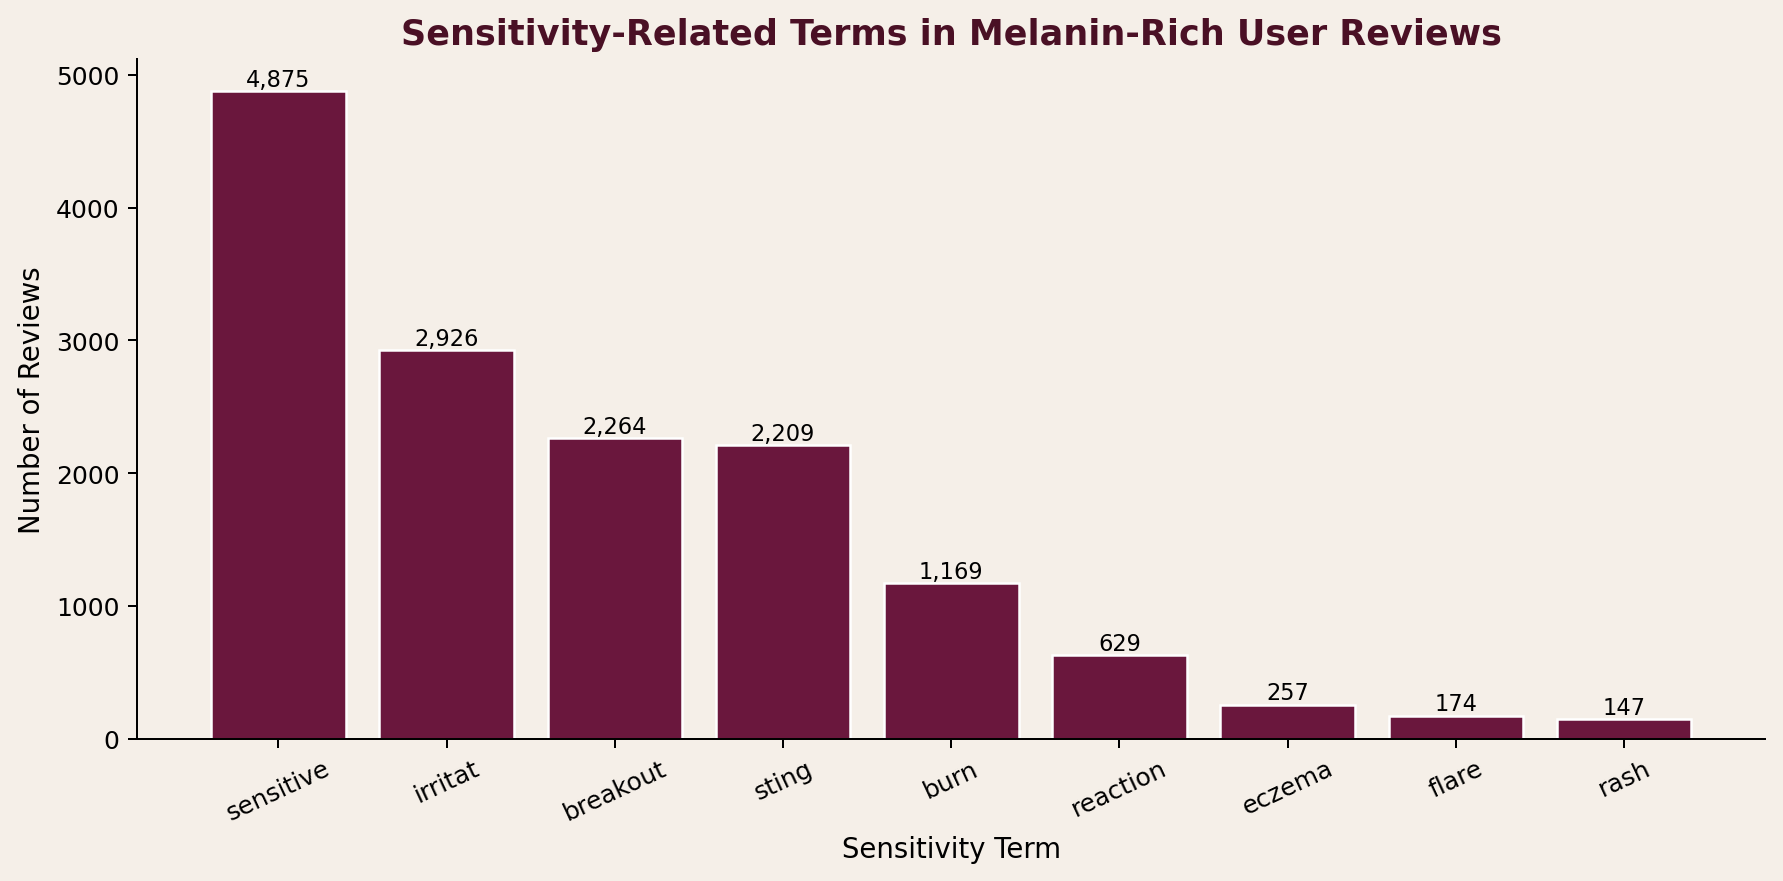
\includegraphics[keepaspectratio]{images/sensitivity_terms.png}}

}

\caption{\label{fig-sensitivity}Sensitivity term frequency in
melanin-rich reviews}

\end{figure}%

When richer and ebony skin tone profiles were selected, the system
showed limited personalized recommendation coverage due to sparse
user-product interaction data in those groups. In those cases, the
system fell back to safety-based recommendations, but personalization
was constrained.

This finding directly demonstrates the tradeoff described in RQ3: adding
safety constraints reduces the candidate pool, and data sparsity for
specific skin tone groups further limits personalized ranking. However,
safety-based recommendations were still produced in all cases.

\subsection{8.4 Prototype
Implementation}\label{prototype-implementation}

The Skintone application was successfully implemented and demonstrated
locally using Streamlit. During deployment to Streamlit Community Cloud,
configuration and data parsing issues prevented the live cloud version
from running consistently. Because the local application remained fully
functional, the final prototype was demonstrated locally. This
deployment issue is treated as an implementation limitation rather than
a failure of the recommender model or application logic.

\textbf{To run locally:}

\begin{Shaded}
\begin{Highlighting}[]
\FunctionTok{git}\NormalTok{ clone https://github.com/sheriannmclarty/Clean\_Beauty\_Recommender\_System}
\BuiltInTok{cd}\NormalTok{ Clean\_Beauty\_Recommender\_System}
\ExtensionTok{pip}\NormalTok{ install }\AttributeTok{{-}r}\NormalTok{ requirements.txt}
\ExtensionTok{streamlit}\NormalTok{ run cb\_app.py}
\end{Highlighting}
\end{Shaded}

\begin{center}\rule{0.5\linewidth}{0.5pt}\end{center}

\section{9. Discussion}\label{discussion}

Skintone demonstrates that beauty recommender systems can be designed to
enforce ingredient safety and surface skin tone compatibility signals
without abandoning personalization. The filter-first architecture
separates safety compliance from ranking logic, making it possible to
guarantee that prohibited ingredients never appear in recommendations
regardless of the underlying model's predictions.

The Skin Tone Review Signal approach revealed an important distinction
between ingredient safety and skin tone compatibility. A product can
pass all ingredient safety screening and still raise skin tone concerns
--- as demonstrated by the sunscreen findings, where mineral SPF
products with zinc oxide consistently received negative tone signals
from melanin-rich reviewers despite being considered safer alternatives
to chemical sunscreens.

One clarification that emerged from the capstone presentation is the
distinction between the Skin Tone Review Signal and a medical or
dermatological safety score. The signal is explicitly a review-based
proxy for visible performance, not a clinical assessment. Future work
should explore whether more robust NLP methods or clinical data could
produce stronger compatibility signals.

The presentation also prompted productive discussion about the
anonymization of reviewer IDs. To make the interface readable while
protecting reviewer identity, encoded reviewer IDs were replaced with
randomly generated display names drawn from a diverse pool representing
Black American, Caribbean, African, Afro-Latina, and South Asian
communities. These display names are not real individuals --- they are
aliases used to make the demo more natural while preserving the
anonymized review profile behind the scenes.

\begin{center}\rule{0.5\linewidth}{0.5pt}\end{center}

\section{10. Limitations}\label{limitations}

\begin{itemize}
\item
  \textbf{Skincare-only dataset:} The 42,715 reviews cover skincare
  products only. Foundation and complexion makeup products are not
  represented, limiting tone-aware recommendations for the category
  where skin tone compatibility is most visible.
\item
  \textbf{Tied predicted ratings:} The bias-adjusted model produces tied
  predicted ratings for users with limited review history. A matrix
  factorization approach such as SVD would produce more differentiated
  predictions.
\item
  \textbf{Ingredient presence vs.~dosage:} EU CosIng screening
  identifies ingredient presence but does not account for dosage or
  concentration risk. SCCS opinions include dosage thresholds but were
  not available for this implementation.
\item
  \textbf{Keyword-based tone signal:} The Skin Tone Review Signal uses
  keyword matching in review text and may miss nuanced language or
  produce false positives.
\item
  \textbf{Sparsity for richer/ebony profiles:} Richer and ebony skin
  tone profiles had limited personalized recommendation coverage due to
  sparse user-product interaction data.
\item
  \textbf{Streamlit Cloud deployment:} The cloud deployment encountered
  data parsing issues and was demonstrated locally. The local app ran
  successfully and demonstrated the full recommendation workflow.
\end{itemize}

\begin{center}\rule{0.5\linewidth}{0.5pt}\end{center}

\section{11. Future Work}\label{future-work}

Phase 3 of the Skintone project will focus on:

\begin{enumerate}
\def\labelenumi{\arabic{enumi}.}
\item
  Adding foundation, concealer, skin tint, tinted moisturizer, BB cream,
  CC cream, and setting powder reviews to support tone-aware
  recommendations for complexion makeup.
\item
  Using the skin tone swatch selector as a stronger recommendation input
  for shade and undertone matching.
\item
  Improving review-text analysis with more robust NLP methods beyond
  keyword-based signals.
\item
  Expanding evaluation with formal metrics including Precision@K,
  NDCG@K, recommendation coverage, and avoid-list violation rate.
\item
  Deploying a stable cloud version with a cleaned, deployment-ready
  dataset.
\item
  Conducting a structured user study with melanin-rich participants to
  assess recommendation relevance, safety confidence, and skin tone
  match confidence.
\end{enumerate}

\begin{center}\rule{0.5\linewidth}{0.5pt}\end{center}

\section{12. Conclusion}\label{conclusion}

Skintone demonstrates how a beauty recommender can move beyond
popularity and average ratings by incorporating ingredient safety, skin
type preferences, and skin tone-aware review signals into the
recommendation pipeline. The prototype showed that a product can be
highly rated and pass ingredient safety screening while still raising
skin tone compatibility concerns --- a distinction that existing
recommenders do not make visible to users.

The system also revealed that personalization depends on representation
in the underlying data. When richer and ebony tone groups had limited
review coverage, the recommender could still support safety-based
filtering, but personalized ranking became limited. This finding
supports the larger purpose of the project: building beauty
recommendation systems that are safer, more transparent, and more
responsive to the needs of melanin-rich users.

Safety and inclusion should be measurable requirements in recommender
systems --- not features added after the fact, and not afterthoughts.
Skintone is a step toward making both visible.

\begin{center}\rule{0.5\linewidth}{0.5pt}\end{center}

\section{References}\label{references}

Collins, M., et al.~(2023). Ingredient safety disparities in personal
care products marketed to Black and brown women. \emph{Environmental
Health Perspectives.}

European Commission. (2026). \emph{CosIng --- Cosmetic Ingredients and
Substances Database.} Annex II and III. Retrieved March 2026 from
https://ec.europa.eu/growth/tools-databases/cosing/

Koren, Y., Bell, R., \& Volinsky, C. (2009). Matrix factorization
techniques for recommender systems. \emph{IEEE Computer, 42}(8), 30--37.

nadyinky. (2023). \emph{Sephora Products and Skincare Reviews.} Kaggle.
https://www.kaggle.com/datasets/nadyinky/sephora-products-and-skincare-reviews

Ricci, F., Rokach, L., \& Shapira, B. (2015). \emph{Recommender Systems
Handbook} (2nd ed.). Springer.

U.S. Food and Drug Administration. (2022). \emph{Modernization of
Cosmetics Regulation Act of 2022 (MoCRA).}
https://www.fda.gov/cosmetics/cosmetics-laws-regulations/modernization-cosmetics-regulation-act-2022-mocra

\begin{center}\rule{0.5\linewidth}{0.5pt}\end{center}

\section{Appendix A: System Architecture
Table}\label{appendix-a-system-architecture-table}

{\def\LTcaptype{none} % do not increment counter
\begin{longtable}[]{@{}
  >{\raggedright\arraybackslash}p{(\linewidth - 6\tabcolsep) * \real{0.2500}}
  >{\raggedright\arraybackslash}p{(\linewidth - 6\tabcolsep) * \real{0.2500}}
  >{\raggedright\arraybackslash}p{(\linewidth - 6\tabcolsep) * \real{0.2500}}
  >{\raggedright\arraybackslash}p{(\linewidth - 6\tabcolsep) * \real{0.2500}}@{}}
\toprule\noalign{}
\begin{minipage}[b]{\linewidth}\raggedright
Layer
\end{minipage} & \begin{minipage}[b]{\linewidth}\raggedright
Component
\end{minipage} & \begin{minipage}[b]{\linewidth}\raggedright
Input
\end{minipage} & \begin{minipage}[b]{\linewidth}\raggedright
Output
\end{minipage} \\
\midrule\noalign{}
\endhead
\bottomrule\noalign{}
\endlastfoot
1 & User Input & Preferences form & Skin tone, skin type, category,
allergen flags \\
2 & EU CosIng Filter & Product ingredients & Blocked / flagged products
removed \\
3 & Allergen Screen & Ingredient strings & Nut-derived products
removed \\
4 & Sensitivity Screen & Review text & High-irritation products
removed \\
5 & CF Ranking & User-item matrix & Predicted ratings \\
6 & Tone Re-rank & Review text scores & Final ranked output \\
7 & Display & Ranked results & Best Matches + Use Caution cards \\
\end{longtable}
}

\section{Appendix B: GitHub
Repository}\label{appendix-b-github-repository}

\textbf{Repository:}
https://github.com/sheriannmclarty/Clean\_Beauty\_Recommender\_System

\textbf{Key files:}

{\def\LTcaptype{none} % do not increment counter
\begin{longtable}[]{@{}ll@{}}
\toprule\noalign{}
File & Purpose \\
\midrule\noalign{}
\endhead
\bottomrule\noalign{}
\endlastfoot
cb\_app.py & Main Streamlit application \\
cb\_tone\_ranking.py & Skin tone review signal computation \\
cb\_bias\_adjusted\_model.py & Bias-adjusted CF model training \\
cb\_inci\_filter.py & EU CosIng ingredient screening \\
requirements.txt & Python dependencies \\
\end{longtable}
}

\section{Appendix C: Sensitivity Term
Frequency}\label{appendix-c-sensitivity-term-frequency}

{\def\LTcaptype{none} % do not increment counter
\begin{longtable}[]{@{}lll@{}}
\toprule\noalign{}
Term & Reviews Mentioning & \% of Dataset \\
\midrule\noalign{}
\endhead
\bottomrule\noalign{}
\endlastfoot
sensitive & 4,875 & 11.4\% \\
irritat & 2,926 & 6.9\% \\
breakout & 2,264 & 5.3\% \\
sting & 2,209 & 5.2\% \\
burn & 1,169 & 2.7\% \\
reaction & 629 & 1.5\% \\
eczema & 257 & 0.6\% \\
flare & 174 & 0.4\% \\
rash & 147 & 0.3\% \\
\end{longtable}
}




\end{document}
